\chapter{3-class \texorpdfstring{$Q$-antipodal}{Q-antipodal}: LSSDs}\label{3class}
In \cite{Cameron1972}, Cameron investigated groups with inequivalent doubly-transitive permutation representations having the same permutation character and introduced the notion of a linked system of symmetric designs (LSSD). One such example arising from Kerdock codes was communicated by Goethals \cite{Goethals1976} and studied in depth by Cameron and Seidel \cite{Cameron1973}. These structures, in the homogeneous case, were then further studied by Noda \cite{Noda1974} who bounded the number of fibers in a LSSD in terms of the design parameters induced between any two of the fibers. Focusing on the $(16,6,2)$ designs, Mathon \cite{Mathon1981} classified all inequivalent LSSDs using these design parameters via a computer search, finding that there were multiple inequivalent LSSDs with two or three fibers but only the scheme described by Geothals worked with four or more fibers. Later, Van Dam proved in \cite{VanDam1999} the equivalence between these objects and 3-class Q-antipodal association schemes. Martin, Muzychuk, and Williford found a connection to mutually unbiased bases in certain dimensions \cite{Martin2007}. Finally Davis, Martin, Polhill \cite{Davis2014} and Jedwab, Li, Simon \cite{Jedwab2017} built more non-trivial examples using difference sets in 2-groups.\par
We begin this chapter with a survey of known results focusing on the connection to association schemes. We introduce ``linked simplices", natural geometric objects which are of interest in their own right, as collections of full-dimensional simplices with only two possible angles between vectors in distinct simplices. We establish the equivalence of sets of linked simplices and LSSDs. We compare three known bounds on the number of fibers and explore connections to structures in Euclidean space. We show how to construct equiangular lines from arbitrary LSSDs and explore cases where LSSDs lead to real mutually unbiased bases (MUBs). After reviewing known examples, we focus on the case of Menon design parameters and, employing an equivalence with sets of mutually unbiased Hadamard matrices, we construct new families of LSSDs for many values of $v$. In particular, we show that one may fix the largest power of two dividing $v$ without bounding the number of fibers in an LSSD, a result which was not previously known. In Appendix \ref{families}, we survey the design parameters of known infinite families of symmetric designs and determine which of these cannot be the design parameters of LSSDs with more than two fibers, noting differences vis-\'{a}-vis a recent discovery by Jedwab et.\ al.\ \cite{Jedwab2017} in restricted cases.

Throughout this chapter we will heavily discuss both the parameters of the association schemes given by LSSDs as well as the design parameters of the given symmetric designs. Thus, for clarity sake, we will always refer to the triple $(v,k,\lambda)$ as the \emph{design parameters} of the LSSD so as to distinguish these from the intersection numbers, Krein parameters, and eigenmatrices of an association scheme. This chapter is based on research published in \cite{Kodalen2019}. Below we list the main theorems of this chapter.
\begin{restatable*}{thm}{lssdsimpequiv}
	A $LSSD(v,k,\lambda;w)$ is equivalent to a set of $w$ linked simplices in $\mathbb{R}^{v-1}$ whose angles depend on the parameters $v$, $k$, and $\lambda$.
\end{restatable*}
\begin{restatable*}{thm}{lssdhadequiv}
	\label{equiv}
	An optimistic $LSSD(v,k,\lambda;w)$ with $\vert v-2k\vert = 2\sqrt{k-\lambda}$ exists if and only if there exists a set of $w-1$ regular unbiased Hadamard matrices, $H_i$, with order $v$ and $H_iJ = 2\sqrt{k-\lambda}J$.
\end{restatable*}
\begin{restatable*}{thm}{buildinghad}[cf.\ Thm~13 in \cite{Kharaghani2010}]
	\label{newLSSD}
	Given a regular Hadamard matrix of order $n$ and an orthogonal array of size $n^2\times N$,
	\begin{itemize}
		\item There exist $N-1$ regular unbiased Hadamard matrices of order $n^2$.
		\item There exists a $LSSD$ with $v=n^2$ and $w=N$.
	\end{itemize}
\end{restatable*}
\begin{restatable*}{cor}{asymplssd}
	\label{asymptotics}
	For sufficiently large $n$, if there exists a regular Hadamard matrix of order $n$, then there exists a $LSSD(n^2,k,\lambda; w)$ with $w \geq n^\frac{1}{14.8}$.
\end{restatable*}
\begin{restatable*}{cor}{oddlssd}
	For any $n\geq 1$ and $w>2$, there exists an odd $t$ for which there exists an $LSSD(16^nt,k,\lambda;w)$.
\end{restatable*}
\begin{restatable*}{cor}{lssdthreesix}
	There exists an $LSSD(v,k,\lambda;w)$ with $v=36^{2n}$ and $w = 4^n+1$ for all $n\geq 1$.
\end{restatable*}
\section{Homogeneous linked systems of symmetric designs}
We begin by reviewing symmetric designs as these will play a central role in all that follows. A \textit{symmetric 2-design}\index{block design!2-design} with design parameters $(v,k,\lambda)$ is a set of blocks $\mathcal{B}$ on point set $X$ written as $(X,\mathcal{B})$ satisfying the following three conditions:
\begin{itemize}
	\item There are $v$ blocks and $v$ points ($\vert\mathcal{B}\vert = \vert X\vert = v$);
	\item Every block contains $k$ points and every point is contained in $k$ blocks;
	\item Every pair of points is contained in $\lambda$ blocks and the intersection of any pair of blocks contains $\lambda$ points.
\end{itemize}
We will ignore the case $v=k=\lambda$ and consider the case $k=1,\lambda=0$ ``degenerate".

We form an \textit{incidence}\index{block design!incidence matrix} matrix $B$ for the block design, indexing rows by blocks and columns by points, setting $B_{ij} = 1$ if point $j$ is in block $i$ and $B_{ij} = 0$ otherwise. Finally, we note the following two equivalent equations which hold for any symmetric 2-design:
\begin{align}
k(k-1) &= \lambda(v-1)\label{sym:1},\\
k(v-k) &= (k-\lambda)(v-1).\label{sym:2}
\end{align}
The \emph{incidence graph} of $(X,\mathcal{B})$ is the graph whose adjacency matrix is $\left[\begin{array}{c:c}
0 & B\\\hdashline[2pt/2pt]
B^T & 0
\end{array}\right].$


We now move to a description of a homogeneous\footnote{Here, ``homogeneous" refers to the designs between fibers all having the same design parameters. For the duration of this chapter, we will only concern ourselves with this case, though we drop this clarification later and refer to the structures simply as linked systems of symmetric designs.} linked system of symmetric designs as described by Cameron in \cite{Cameron1972} and Noda in \cite{Noda1974}. 
Consider a multipartite graph $\Gamma$ on $wv$ vertices with vertex set partitioned into $w$ sets of $v$ vertices called ``fibers":
\[X = X_1\dot{\cup} X_2\dot{\cup}\cdots\dot{\cup}X_w.\]
We say $\Gamma$ is a \emph{linked system of symmetric designs}\index{linked system of symmetric designs}, $LSSD(v,k,\lambda;w)$ ($w\geq 2$), if it satisfies the following three properties:
\begin{enumerate}[label=$(\roman*)$]
	\item no edge of $\Gamma$ has both ends in the same fiber $X_i$;
	\item for all $1\leq i,j\leq w$ with $i\neq j$, the induced subgraph of $\Gamma$ between $X_i$ and $X_j$ is the incidence graph of some $(v,k,\lambda)$-design;
	\item there exist constants $\mu$ and $\nu$ such that for distinct $h,i,j$ ($1\leq h,i,j\leq w$), 
	\begin{equation}\label{munudef}
	a\in X_i, b\in X_j \Rightarrow\vert\Gamma(a)\cap\Gamma(b)\cap X_h\vert=\begin{cases}
	\mu & a\sim b\\
	\nu & a\not\sim b
	\end{cases}
	\end{equation}
\end{enumerate}
where $\sim$ denotes adjacency in $\Gamma$ and $\Gamma(x)$ denotes the neighborhood of vertex $x$. Observe that $\Gamma$ is regular with valency $k(w-1)$. A specific type of LSSD introduced in \cite{Davis2014}, constructed from a \text{linking system of difference sets}\index{linking system of difference sets}, is a LSSD where the symmetric design induced between any two fibers comes from a difference set with the further restriction that the difference sets induced between any pair of three fibers interact in a consistent way. Recently Jedwab, Li, and Simon \cite{Jedwab2017} examined these in more detail, building new examples and proving non-existence results for certain design parameters. However, Mathon \cite{Mathon1981} showed there exist three-fiber LSSDs which do not correspond to linking systems of difference sets, thus we expect there to be many LSSDs which we cannot build via linking difference sets. We will consider the general case, and thus do not assume this added structure on our symmetric designs.\par
In \cite[Proposition 0]{Noda1974}, Noda shows that $\mu$ and $\nu$ must take one of two pairs of values given by:
\begin{equation}
\nu = \frac{k(k\pm \sqrt{k-\lambda})}{v}, \qquad \mu = \nu\mp \sqrt{k-\lambda}. \label{mu-nu}
\end{equation}
With these two possibilities for $\mu$ and $\nu$, it becomes useful to distinguish between the two types of LSSDs. We will refer to the LSSD as \emph{$\mu$-heavy}\index{$\mu$-heavy} (resp., \emph{$\nu$-heavy}\index{$\nu$-heavy}) when $\mu>\nu$ (resp., $\nu>\mu$). Note that since both $\mu$ and $\nu$ are integers, we must also have $\sqrt{k-\lambda}\in\bbZ$; for the remainder of this chapter, define $s = \sqrt{k-\lambda}$ Note, this parameter is known as the ``order" of the symmetric design and many authors use $n$ to denote this value --- we will always use $s$. Further, since $k\neq \lambda$, we must have $s>0$ and thus $\mu\neq \nu$. We now review a proposition of Noda which notes that, given an LSSD $\Gamma$, swapping adjacency between fibers produces another LSSD; we call this graph the \emph{multipartite complement} of $\Gamma$.
\begin{prop}[Noda]\label{complement}
	Let $\Gamma$ be a  $LSSD(v,k,\lambda;w)$ with $w>2$. If $\Gamma$ is $\mu$-heavy (resp., $\nu$-heavy), the multipartite complement $\Gamma'$ is a $\nu$-heavy (resp., $\mu$-heavy) $LSSD(v,v-k,v-2k+\lambda;w)$.
\end{prop}
We further find that, given $v$, $k$, and $\lambda$, only one of the outcomes in \eqref{mu-nu} is possible for $v\geq 3$.
\begin{lem}
	\label{gcd}
	Let $\Gamma$ be a  $LSSD(v,k,\lambda;w)$ with $w>2$ and $1<k<v-1$. Then the following hold:
	\begin{enumerate}[label=$(\roman*)$]
		\item exactly one of $\frac{k(k+ s)}{v}$ and $\frac{k(k-s)}{v}$ is an integer;
		\item $\gcd(k,v)>1$;
		\item $\gcd(s,v)>1$.
	\end{enumerate}
\end{lem}
\begin{proof}
	By Proposition $\ref{complement}$, we may assume $k\leq \frac{v}{2}$ as $\frac{k(k\pm s)}{v}$ is integral if and only if $\frac{(v-k)((v-k)\pm s)}{v}$ is integral. Now, Equation \eqref{sym:1} gives $k^2-s^2 = \lambda v$ and thus we have the equations
	\[\begin{aligned}
	\frac{k(k+ s)}{v} -\frac{s(k+ s)}{v} =\frac{k(k- s)}{v} +\frac{s(k- s)}{v} &= \lambda.
	\end{aligned}\]
	Now assume $\frac{k(k+s)}{v}$ and $\frac{k(k-s)}{v}$ are both integral. This implies that $\frac{s(k+s)}{v}$ and $\frac{s(k-s)}{v}$ are both integral, and thus their difference $\frac{2s^2}{v}$ must also be integral. However this contradicts $s<k\leq\frac{v}{2}$, thus at most one of $\frac{k(k+s)}{v}$ and $\frac{k(k-s)}{v}$ may be integral. The assumption that our parameters were feasible (in fact, realizable) is sufficient to guarantee at least one is an integer, giving $(i)$. For $(ii)$, we again assume $k\leq \frac{v}{2}$ (noting that $\gcd(k,v) = \gcd(v-k,v)$ since $k<v$). Now, since $s<k$ we must have $k+s<v$. Thus if $\frac{k(k+s)}{v}$ is an integer, we must have $\gcd(k,v)>1$. Similarly $\frac{k(k-s)}{v}\in\mathbb{Z}$ implies $\gcd(k,v)>1$. The same argument applies to $(iii)$ noting again that one of $\frac{k(k\pm s)}{v}$ is integral if and only if one of $\frac{s(k\pm s)}{v}$ is integral.
\end{proof}
\begin{remark}
	\label{rmk1}
	Theorem \ref{Qpoly} and the discussion that follows shows that the parameters of an LSSD uniquely determine the parameters of an association scheme. It is important to note here that the first line of Lemma \ref{gcd} may be replaced with the line ``Suppose the parameter set of a $LSSD(v,k,\lambda;w)$ with $w>2$ and $1<k<v-1$ is feasible." In fact, all we need to prove Lemma \ref{gcd} is that either $\frac{k(k+s)}{v}$ or $\frac{k(k-s)}{v}$ is integral. This will become useful as we apply this lemma to rule out feasible parameter sets where, clearly, we cannot assume the LSSD exists.
\end{remark}
The case where $k=1$ or $k=v-1$ produces LSSDs which are not of interest to us and for the remainder of the chapter, we will refer to these designs as ``degenerate". For a further description of why these designs are degenerate, see Section \ref{degenerate}. The observations that $\gcd(k,v)>1$ and $\gcd(s,v)>1$ are two tools which help us determine more easily which design parameters might be feasible for a LSSD with $w>2$. We may find many other statements similar to these, but these two will be sufficient for now. Using these, we can immediately rule out many design parameters. For instance:
\begin{cor}
	\label{comp}
	Assume $w>2$. If there exists a non-degenerate $LSSD(v,k,\lambda;w)$, then $v$ is composite.\qed
\end{cor}
For a further use of these tools to rule out certain families of symmetric designs, see Appendix \ref{families}.

We now provide a theorem of Van Dam concerning the equivalence between linked systems of symmetric designs and 3-class $Q$-antipodal association schemes. We do not give a self-contained proof here, instead referring to results of Van Dam to outline the proof. While this result appears in \cite{VanDam1999}, we include a later result appearing in \cite{vanDam2013} to assist with our outline.
\begin{thm}[\cite{VanDam1999}]
	\label{Qpoly}
	Let $\Gamma$ be a non-degenerate LSSD with adjacency matrix $A$. Then the algebra $\langle A\rangle_*$ is the Bose-Mesner algebra of a 3-class Q-antipodal association scheme on $X$. Conversely, every $Q$-antipodal 3-class association scheme arises in this way. More specifically, the natural ordering of the relations of any $Q$-antipodal 3-class association scheme is as follows:
	\begin{itemize}
		\item $R_0$ is the identity relation on $X$;
		\item $R_1$ is given by adjacency in the $\mu$-heavy LSSD;
		\item $R_2$ is the union of complete graphs on the fibers induced by $R_1$;
		\item $R_3$ is given by adjacency in the $\nu$-heavy LSSD.
	\end{itemize}
\end{thm}
%\begin{proof}
\noindent \textit{Proof outline.} Let $\Gamma$ be the graph of a linked system of symmetric designs with $0<\lambda<k-1$ and assume without loss of generality that $k\leq \frac{v}{2}$. Using the definition of an LSSD, one may verify quickly that all intersection numbers are well-defined, and thus the adjacency algebra of $\Gamma$ is the Bose-Mesner algebra of a 3-class association scheme. We may then build $L_1$ to find that the eigenvalues of this graph are $k(w-1)>\sqrt{k-\lambda}(w-1)>-\sqrt{k-\lambda}>-k$ with multiplicities $m_0,m_1,m_2,m_3$ respectively. Since $\Gamma$ is connected, we find that $m_0=1$. Further, since $\Gamma$ has four distinct eigenvalues, Theorem 5.8 of \cite{VanDam1999} tells us $m_1 = v-1$. We then use the equations $\sum_{i=0}^3\theta_im_i = 0$ and $\sum_{i=0}^3 m_i = vw$ to find that $m_3 = w-1$ and $m_2 = (w-1)(v-1)$. We then apply Proposition 6.1 of \cite{vanDam2013} to see that this association scheme is $Q$-antipodal. Conversely, let $(X,\mathcal{R})$ be a 3-class $Q$-antipodal association scheme with relations ordered naturally. Then Theorem \ref{suzukiimprim} tells us the system of imprimitivity is given by $\mathcal{J} = \left\{0,3\right\}$ and $\mathcal{I} = \left\{0,2\right\}$ and Theorem 5.1 of \cite{vanDam2013} tells us $(X,\mathcal{R})$ is uniform. We may then refer again to Proposition 6.1 of \cite{vanDam2013} to see that $m_2 = (w-1)m_1$. This, along with the antipodal property, forces $k_1 = v-1$ where $k_1$ is the valency of the nearest neighbor graph. Thus Theorem 5.8 of \cite{VanDam1999} tells us this nearest neighbor graph is the incidence graph of a linked system of symmetric designs with $0<\lambda<k-1$.\qed
%\end{proof}
In addition to the above proof, we list the intersection numbers, the first and second eigenmatrices, and a some of the Krein parameters for later use. Let $\Gamma_1 = (X,R_1)$ be a $\mu$-heavy $LSSD(v,k,\lambda)$ with complement design given by $\Gamma_2 = (X,R_3)$. The following are the intersection numbers, listed via the four matrices $L_0,L_1,L_2,L_3$ where $L_i = [p_{i,j}^k]_{k,j}$;
\[\begin{aligned}
L_0 &= \left[\begin{array}{cccc}
1 & 0 & 0 & 0\\
0 & 1 & 0 & 0\\
0 & 0 & 1 & 0\\
0 & 0 & 0 & 1\\
\end{array}\right], \qquad L_1 = \left[\begin{array}{cccc}
0 & k(w-1)       & 0   & 0               \\
1 & \mu(w-2)     & k-1 & (k-\mu)(w-2)    \\
0 & \lambda(w-1) & 0   & (k-\lambda)(w-1)\\
0 & \nu(w-2)     & k   & (k-\nu)(w-2)    \\
\end{array}\right],\\
L_2 &= \left[\begin{array}{cccc}
0 & 0   & v-1 & 0    \\
0 & k-1 & 0   & v-k  \\
1 & 0   & v-2 & 0    \\
0 & k   & 0   & v-k-1\\
\end{array}\right],
\\ L_3 &= \left[\begin{array}{cccc}
0 & 0             & 0     & (v-k)(w-1)\\
0 & (k-\mu)(w-2)  & v-k   & (v+\mu-2k)(w-2)\\
0 & (k-\lambda)(w-1) & 0     &(v+\lambda-2k)(w-1)\\
1 & (k-\nu)(w-2)  & v-k-1 & (v+\nu-2k)(w-2)\\
\end{array}\right].\\
\end{aligned}\]
We note here that, while $\mu$ and $\nu$ alone are not intersection numbers of our association scheme, we will often allow for the slight abuse of terminology and include both of these as parameters of an LSSD. The first and second eigenmatrices are given as:
\begin{equation}\label{3classP}
P = \left[\begin{array}{cccc}
1&k(w-1)&v-1&(v-k)(w-1)\\
1&\sqrt{k-\lambda}(w-1)&-1&-\sqrt{k-\lambda}(w-1)\\
1&-\sqrt{k-\lambda}&-1&\sqrt{k-\lambda}\\
1&-k&v-1&k-v\\
\end{array}\right]
\end{equation}
\begin{equation}\label{3classQ}Q = \left[\begin{array}{cccc}
1 & v-1 & (w-1)(v-1) & w-1\\
1 & \frac{v-k}{\sqrt{k-\lambda}} & -\frac{v-k}{\sqrt{k-\lambda}} & -1\\
1 & -1 & 1-w & w-1\\
1 & \frac{-k}{\sqrt{k-\lambda}} & \frac{k}{\sqrt{k-\lambda}} & -1\\
\end{array}\right].
\end{equation}
Finally, we use this matrix $Q$ to calculate our Krein parameters using standard techniques (see \cite{Brouwer1989}). Defining $L_i^* = [q_{ij}^k]_{k,j}$ similar to before, we find
\[\scalebox{.9}{$L_1^* = \left[\begin{array}{cccc}
0 & v-1 & 0 & 0\\
1 & \frac{(1-w)(2k-v)+(v-2)s}{ws} &\frac{(w-1)\left(s(v-2)+(2k-v)\right)}{ws}& 0\\
0&\frac{s(v-2)+2k-v}{ws} & \frac{s(w-1)(v-2)-(2k-v)}{ws}& 1\\
0& 0 & v-1& 0\\
\end{array}\right],\quad L_3^*=\left[\begin{array}{cccc}
0&0 &0 & w-1\\
0& 0& w-1& 0\\
0& 1& w-2& 0\\
1& 0& 0& w-2\\
\end{array}\right].$}\]
Note that our $Q$-polynomial property means that $L_1^*$ must be irreducible tridiagonal (\cite[Prop.~2.7.1(i')]{Brouwer1989}). While the tridiagonal property is clear from the above matrix, the irreducible property requires $s(v-2)>v-2k$, for which $k>1$ is necessary (and sufficient). Thus, while we may fulfill the LSSD conditions using \emph{degenerate design parameters}\index{degenerate parameters} $(v,1,0)$, these will not satisfy our $Q$-polynomial property. This is one reason why we will ignore this case for much of our discussion.

Finally, the final column of $L_3^*$ tells us that $E_3\circ E_3\in\left<E_0,E_3\right>$; that is, our scheme is $Q$-antipodal. We henceforth use the term \emph{linked system of symmetric designs}\index{linked system of symmetric designs} to refer to either the graph $\Gamma$ or to the association scheme it generates as in Theorem \ref{Qpoly}.
\subsection{Bounds on number of fibers}
\index{Noda bound}
One central question in the study of linked systems of symmetric designs is determining the maximum number of fibers one may use to build LSSDs. Theorem 2 of \cite{Noda1974} provides us with the main non-trivial bound known to date. In this paper, Noda proves
\begin{equation*}\resizebox{\textwidth}{!}{
	$(w-1)\left[(k-2)\lambda\binom{k}{3}-(v-2)\left[(v-k)\binom{\nu}{3} + k\binom{\mu}{3}\right]\right]\leq(v-2)\left[(v-1)\binom{\lambda}{3}+\binom{k}{3}-\left[(v-k)\binom{\nu}{3} + k\binom{\mu}{3}\right]\right]$
}\end{equation*}
with equality if and only if a pair $(X_1,X_2\cup X_3\cup\dots\cup X_w)$ forms a 3-design. If we restrict ourselves to the case of $\mu$-heavy LSSDs, this results in the following theorem
\begin{thm}
	Suppose there exists a $LSSD(v,k,\lambda;w)$ with $\nu = \frac{k(k-s)}{v}$ and $\mu = \nu+s$. Then if $k>\frac{v}{2}$,
	\begin{equation}\label{Noda}w \leq \frac{(v-2)\sqrt{k-\lambda}}{2k-v}+1.\end{equation}
\end{thm}
Note the condition becomes vacuous when $2k<v$, thus the bound only applies when $(2k-v)(\mu-\nu)>0$.

Examining the Krein parameters which arise (in particular those listed in the discussion following Theorem \ref{Qpoly}), we find that the only non-trivial condition from the Krein conditions is $q^1_{11}\geq 0$. While constructing the various different possible configurations of LSSDs using design parameters $(16,6,2)$ \cite{Mathon1981}, Mathon also shows that the condition $q^1_{11}\geq 0$ is equivalent to the Noda bound (seen above). In fact, we have
\begin{equation}\label{q111}
q_{11}^1 =\frac{(1-w)(2k-v)+(v-2)s}{ws}.
\end{equation}
Thus, as long as $k<\frac{v}{2}$ we may rearrange the terms to get
\[w\leq \frac{(v-2)s}{2k-v}+1.\]
This is, of course, equivalent to the previous bound since $s = \sqrt{k-\lambda}$. Note that, as before, we only arrive at this bound if $k<\frac{v}{2}$ for the $\mu$-heavy design.

The final bound we will consider is one which does not require $k<\frac{v}{2}$ for the $\mu$-heavy design. In \cite{Martin2007}, Martin, Muzychuk, and Williford use the absolute bound to bound the number of fibers, relying on the $Q$-polynomial structure (particularly that $q_{11}^3 = 0$ and $q_{11}^2 >0$). Let $m_i = \text{rank}(E_i)$. We know from our $Q$ matrix that $m_2 = (w-1)m_1$. Further,
\begin{equation}\label{abslssd}E_1\circ E_1 = \frac{1}{\vert X\vert}\left(q_{11}^0E_0 + q_{11}^1E_1+q_{11}^2E_2\right).\end{equation}
The bound itself will depend on whether or not $q^1_{11}$ is non-zero. Thus we must split our derivation into two cases. In what follows, we derive the bound for the case $q^1_{11}>0$ as well as examine further the case of $q^1_{11}=0$, deriving the absolute bound for this case and pairing this with tightness in the Noda bound to further restrict our parameters.

First consider the case when $q^1_{11}>0$. Here, we find the rank of the right hand side of \eqref{abslssd} is $m_2+m_1+1$ while the rank on the left is no larger than $\frac{1}{2}m_1\left(m_1+1\right)$. Thus we must have
\[\begin{aligned}
m_2+m_1+1&\leq \frac{1}{2}m_1(m_1+1)\\
(w-1)m_1 &\leq \frac{m_1^2-m_1}{2}-1,\\
w&\leq \frac{m_1-1}{2}-\frac{1}{m_1}.
\end{aligned}\]
Since $m_1 = v-1$, this gives $w \leq \frac{v}{2}-\frac{1}{v-1}$. Further, since $v>2$ this results in $w\leq\frac{v-1}{2}$. 

Now consider the case where $q_{11}^1=0$. The only change is that the right hand side of \eqref{abslssd} now has rank $m_2+1$. Thus our bound gives instead $w\leq \frac{v+1}{2}$. However, \eqref{q111} gives us an expression for $q^1_{11}$. Thus, if $q^1_{11}=0$, we must have $k>\frac{v}{2}$ and $w = \frac{(v-2)s}{2k-v}+1$. Using this value for $w$ in our bound $w\leq \frac{v+1}{2}$ results in the inequality $\frac{(v-2)s}{2k-v}+1\leq \frac{v+1}{2}$ or equivalently, 
\[2s\leq (2k-v) + \frac{2s}{v-1}.\]
Since $0<2s<k<v-1$, we must then have $2s\leq (2k-v)$. Squaring both sides then gives
$4(k-\lambda)\leq 4k^2-4kv+v^2$. Finally, using Equation \eqref{sym:2} we have
\[\begin{aligned}
4(k-\lambda)\leq v.
\end{aligned}\]

In summary, if $q^1_{11}>0$, the absolute bound tells us $w\leq \frac{v-1}{2}$ for both $\mu$-heavy and $\nu$-heavy designs independent of the size of $k$. Additionally, if $q^1_{11}=0$ (i.e.\ the Noda bound is tight), we must have $4(k-\lambda)\leq v$. Recall this is exactly the case where Noda showed $(X_1,X_2\cup X_3\cup\dots\cup X_w)$ forms a 3-design. There is only one known family of constructions which achieve the Noda bound. For this construction (see Section \ref{kerdock}) $v = 4(k-\lambda)$. Further, these designs have parameters belonging to the Menon family --- the only possible family for which this $v=4(k-\lambda)$.

We finish this section by noting that, in either case ($q^1_{11}>0$ and $q^1_{11}=0$), the exact bound arising from the absolute bound is non-integral assuming $m_1>2$. Thus, while we reduce these bounds to $w\leq\frac{v-1}{2}$ and $w\leq\frac{v+1}{2}$, the actual absolute bound will never be tight.


\section{Linked simplices}
\label{linked simplices}
In this section, we will write $\left\{b_j\right\}$ for the set $\left\{b_1,\dots,b_v\right\}$ for both sets of points and sets of blocks. For our purposes a \emph{regular simplex}\index{regular simplex} will be taken to be a set of $v$ unit vectors spanning $\mathbb{R}^{v-1}$ with the property that the inner product of any pair of distinct vectors is $-\frac{1}{v-1}$. Let $\mathcal{A} = \left\{a_i\right\}$ and $\mathcal{B} = \left\{b_j\right\}$ be two regular simplices in $\mathbb{R}^{v-1}$. We say $\mathcal{A}$ and $\mathcal{B}$ are \emph{linked}\index{linked simplices} if there exist two real numbers $\gamma$ and $\delta$ such that for all $1\leq i,j\leq v$, $\left<a_i,b_j\right>\in \left\{\gamma,\delta\right\}$. (Note that, here, ``linked" always implies regular.) Following the same abuse of terminology as we did with equiangular lines in Chapter \ref{psdcone}, we will refer to the real numbers $\gamma$ and $\delta$ as the ``angles" of our linked simplices. Extending this, given regular simplices $\mathcal{A}_1,\dots,\mathcal{A}_w$ in $\mathbb{R}^{v-1}$ we say $\left\{A_1,\dots,A_w\right\}$ is a \emph{set of $w$ linked simplices} if any two of them are linked with the same angles $\gamma$ and $\delta$. The next few theorems establish an equivalence between these objects and LSSDs. 
\begin{thm}
	\label{Association2Simplex}
	Consider a $LSSD(v,k,\lambda;w)$ with Bose-Mesner algebra $\mathbb{A}$. The first idempotent $E_1$ in a $Q$-polynomial ordering of $\mathbb{A}$, appropriately scaled, is the Gram matrix of a set of $w$ linked simplices. In the case $w=2$, $E_2$ scaled similarly is also the Gram matrix of a second set of two linked simplices.
\end{thm}
\begin{proof}
	Let $(X,\mathcal{R})$ be a $LSSD(v,k,\lambda;w)$ with Bose-Mesner algebra $\mathbb{A}$. Let $\left\{A_i\right\}$ and $\left\{E_j\right\}$ be the bases of Schur and matrix idempotents respectively. We have from \eqref{PQmat}
	\[E_j = \frac{1}{\vert X\vert}\sum Q_{ij}A_i.\]
	As $E_j$ is an idempotent, $E_j$ is a positive semidefinite matrix with rank $Q_{0j}$. Therefore using \eqref{3classQ},
	\[G = \frac{vw}{v-1}E_1 = A_0 + \frac{v-k}{(v-1)\sqrt{k-\lambda}}A_1 -\frac{1}{v-1}A_2 -\frac{k}{(v-1)\sqrt{k-\lambda}}A_3\]
	is positive semidefinite with 1 on the main diagonal. Given that $Q_{01} = v-1$, $G$ is the Gram matrix of a set $Y$ of $vw$ vectors in $\mathbb{R}^{v-1}$. Further there are only three possible inner products among distinct vectors of $Y$ given by
	\[\alpha_1 = \frac{v-k}{(v-1)\sqrt{k-\lambda}},\qquad\alpha_2 =-\frac{1}{v-1},\qquad\alpha_3 = -\frac{k}{(v-1)\sqrt{k-\lambda}}.\]
	Since $A_2$ has the form $I_w\otimes J_v$, encoding adjacency in the complete graphs within fibers, our vectors form a set of $w$ linked simplices in $\mathbb{R}^{v-1}$ with $\gamma = \alpha_1$ and $\delta = \alpha_3$ as inner products between vectors in distinct simplices.\par
	Similarly we have
	\[\begin{aligned}
	G' = \frac{vw}{v-1}E_2 &= \left(A_0 + \frac{-k}{(v-1)\sqrt{k-\lambda}}A_1 -\frac{1}{v-1}A_2 +\frac{v-k}{(v-1)\sqrt{k-\lambda}}A_3\right)\\
	\end{aligned}\]
	forcing $G'$ also to be the Gram matrix of a set of vectors coming from $w$ distinct simplices. However, the rank of $E_2$ is $(w-1)(v-1)$ and thus these simplices are full-dimensional, hence linked, only when $w=2$. This means any pair of fibers from our LSSD will give us another set of linked simplices with inner products $-\alpha_1$ and $-\alpha_3$. This corresponds to choosing one of the two simplices and replacing each $x$ in that simplex by $-x$.
\end{proof}
This tells us that every LSSD gives rise to a set of linked simplices. Before proving the converse, we first prove a lemma arising from the observation that a regular simplex is an equiangular tight frame\index{equiangular tight frame}, that is, a set of vectors $\left\{v_j\right\}_{j\in J}\subset V$ for which there exists a constant $A$ so that $v = \frac{1}{A}\sum_{j\in J} \left<v,v_j\right>v_j$ for every vector $v\in V$. We will instead use the equivalent Plancherel definition $\left<v,w\right> = \frac{1}{A}\sum_{j\in J}\left<v,v_j\right>\left<v_j,w\right>$ for all $v,w\in V$ (see \cite{Jasper2014}).
\begin{lem}
	\label{simplextobasis}
	Let $\left\{a_i\right\}$ be a regular simplex in $\mathbb{R}^{v-1}$ and let $x,y\in \mathbb{R}^{v-1}$. Then
	\[\begin{aligned}
	\sum_i \left<a_i,x\right>\left<a_i,y\right> = \frac{v}{v-1}\left<x,y\right>.
	\end{aligned}\]
\end{lem}
\begin{proof}
	For a vector $x$, let $x(i)$ denote the $i^\text{th}$ entry of $x$. For each $1\leq i\leq v$, define $\alpha_i\in \mathbb{R}^{v}$ as the unit vector
	\[\alpha_i = \sqrt{\frac{v-1}{v}}\left[a_i(1),a_i(2),\dots,a_i(v-1),\frac{1}{\sqrt{v-1}}\right].\]
	For $i\neq i^\prime$,
	\[\left<\alpha_i,\alpha_{i^\prime}\right> = \frac{v-1}{v}\left(\left<a_i,a_{i^\prime}\right> + \frac{1}{v-1}\right)=0.\]
	Then $\left\{\alpha_i\right\}$ forms an orthonormal basis for $\mathbb{R}^v$. Now define $\chi,\psi\in\mathbb{R}^v$ as:
	\[\chi = \left[x(1),x(2),\dots,x(v-1),0\right],\qquad\psi = \left[y(1),y(2),\dots,y(v-1),0\right].\]
	Then for each $i$,
	\[\begin{aligned}
	\left<\alpha_i, \chi\right> = \sqrt{\frac{v-1}{v}}\left<a_i,x\right>,\qquad\left<\alpha_i, \psi\right> = \sqrt{\frac{v-1}{v}}\left<a_i,y\right>
	\end{aligned}\]
	giving us
	\[\left<x,y\right> =\left<\chi,\psi\right>=\sum_i\left<\alpha_i, \chi\right>\left<\alpha_i, \psi\right> =\frac{v-1}{v}\sum_i\left<a_i,x\right>\left<a_i,y\right>.\qedhere\]
\end{proof}
Using this lemma, we now seek to build a LSSD with $w$ fibers from a set of $w$ linked simplices. We first provide a construction of the graph $\Gamma$ and then split the verification into two parts: first that $\Gamma$ restricted to a pair of fibers represents a symmetric design, and second that the constants $\mu$ and $\nu$ given by \eqref{munudef} are well-defined. Clearly, we need only consider three fibers in the proofs to follow; the arguments extend to $w$ fibers.
\begin{thm}
	\label{2design}
	Let $\left\{a_i\right\}$ and $\left\{b_j\right\}$ be linked simplices in $\mathbb{R}^{v-1}$ with inner products $\gamma$ and $\delta$. For each $j$, let $B_j = \left\{a_i:\left<a_i,b_j\right> = \gamma\right\}$. Then $(\left\{a_i\right\},\left\{B_j\right\})$ is a symmetric 2-design.
\end{thm}
\begin{proof}
	First we must prove that each block contains a constant number of points. Let $1\leq j\leq v$ be fixed and define $k_j = \vert B_j\vert$. Since the set $\left\{a_i\right\}$ of vectors form a regular simplex, the centroid of those vectors must be the origin. Then, $\sum_i\left<b_j,a_i\right> = \left<b_j,\sum_ia_i\right> = 0$ giving us the equation $k_j\gamma + (v-k_j)\delta = 0$. Solving this for $k_j$ gives $k_j = \frac{\delta v}{\gamma-\delta}$, independent of $j$. Now we will show that any pair of blocks have a constant number of points in common; swapping roles this gives that any pair of points is contained in a constant number of blocks. Fix $1\leq s,t\leq v$ so that $b_s$ and $b_t$ are two distinct vectors in $\left\{b_j\right\}$ with corresponding blocks $B_s$ and $B_t$ respectively. Define $\lambda_{s,t} = \vert B_s\cap B_t\vert$ and
	\[x_s = \left[\left<a_1,b_s\right>,\left<a_2,b_s\right>,\dots,\left<a_v,b_s\right>\right],\qquad x_t = \left[\left<a_1,b_t\right>,\left<a_2,b_t\right>,\dots,\left<a_v,b_t\right>\right].\]
	Recalling that $k\gamma+(v-k)\delta = 0$,
	\[\left<x_s,x_t\right> = \lambda_{s,t} \gamma^2 + 2(k-\lambda_{s,t})\gamma\delta + (v-2k+\lambda_{s,t})\delta^2=\lambda_{s,t}\left(\delta-\gamma\right)^2 - v\delta^2.\]
	We may instead apply Lemma \ref{simplextobasis} to get
	\[\left<x_s,x_t\right> = \sum_i \left<a_i,b_s\right>\left<a_i,b_t\right>=\frac{v}{v-1}\left<b_s,b_t\right>=-\frac{v}{(v-1)^2}.\]
	Equating these two values gives us
	\[\lambda_{s,t} =\frac{v\delta^2}{(\delta-\gamma)^2}-\frac{v}{(v-1)^2(\gamma-\delta)^2}.\]
	The quantity on the right is independent of $s$ and $t$ and therefore $\lambda_{s,t}$ does not depend on $s$ and $t$. This tells us our collection of blocks forms a $2$-design with the above values for $k$ and $\lambda$.
\end{proof}
As both $k$ and $\lambda$ are integers, this gives us restrictions on which inner products are allowed. We solve the system
\[\begin{aligned}
k\gamma + (v-k)\delta &= 0,\\
\lambda(\delta-\gamma)^2 - v\delta^2 &= -\frac{v}{(v-1)^2}\\
\end{aligned}\]
to find that $\delta^2 =\frac{k}{(v-1)(v-k)}$. Using \eqref{sym:2}, this simplifies to
\begin{equation}\label{angles}
\delta = \pm\frac{k}{(v-1)\sqrt{k-\lambda}},\qquad\gamma = \mp\frac{v-k}{(v-1)\sqrt{k-\lambda}}.
\end{equation}
These match the previously determined entries of $E_1$ and $E_2$ corresponding to the first and third relations. Our next theorem concerns the existence of $\mu$ and $\nu$, which arise between triples of fibers.
\begin{thm}
	\label{3fibers}
	Let $\left\{a_i\right\}$, $\left\{b_i\right\}$, and $\left\{c_i\right\}$ be three linked simplices in $\mathbb{R}^{v-1}$ with inner products $\gamma$ and $\delta$ as before. For each $1\leq j,k\leq v$, let $B_j = \left\{a_i:\left<a_i,b_j\right> = \gamma\right\}$ and $C_k = \left\{a_i:\left<a_i,c_k\right> = \gamma\right\}$. Then there exists integers $\mu$ and $\nu$ such that 
	\[\vert B_j\cap C_k\vert = \begin{cases}
	\mu  & \left<b_j,c_k\right> = \gamma\\
	\nu  & \left<b_j,c_k\right> = \delta\\
	\end{cases}\]
	where $\mu$ and $\nu$ are independent of our choice of $j$ and $k$.
\end{thm}
\begin{proof}
	We follow a similar method of calculating an inner product in two ways, then equating the results. Fix $0\leq i,j\leq v$ and let $\eta_{i,j} = \vert B_i\cap C_j\vert$. Define
	\[x_i = \left[\left<a_1,b_i\right>,\left<a_2,b_i\right>,\dots,\left<a_v,b_i\right>\right],\qquad x_j = \left[\left<a_1,c_j\right>,\left<a_2,c_j\right>,\dots,\left<a_v,c_j\right>\right].\]
	Then we have $\left<x_i,x_j\right> =\eta_{i,j}(\gamma-\delta)^2 - v\delta^2$ and using Lemma \ref{simplextobasis},
	\[\left<x_i,x_j\right> = \sum_\ell \left<a_\ell,b_i\right>\left<a_\ell,c_j\right>=\frac{v}{v-1}\left<b_i,c_j\right>.\]
	Equating these two values and solving for $\eta_{i,j}$ gives us
	\[\eta_{i,j} = \frac{1}{(\gamma-\delta)^2}\left(v\delta^2 + \frac{v}{v-1}\left<b_i,c_j\right>\right).\]
	While the right side is not independent of $i$ and $j$ as we saw in the previous theorem, it is only dependent on the value of $\left<b_i,c_j\right>$. Using $\nu$ and $\mu$ for $\eta_{i,j}$ when $\left<b_i,c_j\right>$ is $\delta$ and $\gamma$ respectively, we have
	\[\begin{aligned}
	\nu&=\frac{v}{(\gamma-\delta)^2}\left(\frac{\delta^2(v-1)^2+\delta(v-1)}{(v-1)^2}\right),\\
	\mu&=\frac{v}{(\gamma-\delta)^2}\left(\frac{\delta^2(v-1)^2+\gamma(v-1)}{(v-1)^2}\right)= \nu + \frac{v}{(\gamma-\delta)(v-1)}.
	\end{aligned}\]
	Using equation \ref{angles}, we find
	\[\begin{aligned}
	\gamma-\delta&=\mp\frac{v}{(v-1)\sqrt{k-\lambda}},
	\end{aligned}\]
	giving us that
	\[\begin{aligned}
	\nu&= \frac{k(k\pm \sqrt{k-\lambda})}{v},\\
	\mu&=\nu\mp\sqrt{k-\lambda}.\qedhere
	\end{aligned}\]
\end{proof}
Note that, since $\mu$ and $\nu$ are both cardinalities of sets, any time we find non-integral values for $\mu$ and $\nu$ we can conclude that the hypothesized set of linked simplices does not exist. This brings us to the main theorem of this section (cf.\ \cite[Theorem~2.6(1)]{Suda2011}).
\lssdsimpequiv
%\begin{thm}
%	A $LSSD(v,k,\lambda;w)$ is equivalent to a set of $w$ linked simplices in $\mathbb{R}^{v-1}$.
%\end{thm}
\begin{proof}
	Theorem \ref{Association2Simplex} tells us that given any $LSSD(v,k,\lambda;w)$ we can always build a set of $w$ linked simplices using a scaled version of the first idempotent as the Gram matrix. For the converse, let $\left\{X_1,X_2,\dots,X_w\right\}$ be a set of $w$ linked simplices with inner products $\gamma>\delta$. Define a graph $\Gamma$ on vertex set $\bigcup_i X_i$ where $x\in X_j$ and $y\in X_\ell$ ($j\neq \ell$) are adjacent if and only if $\left<x,y\right> = \gamma$. Then $\Gamma$ is a multipartite graph with $w$ fibers. Theorem \ref{2design} tells us that the induced graph between a pair of fibers is a symmetric $2$-design. Theorem $\ref{3fibers}$ shows that given any pair of vertices in distinct fibers $x\in X_i$ and $y\in X_\ell$,
	\[\vert\Gamma(x)\cap\Gamma(y)\cap X_j\vert = \begin{cases}
	\mu & x\sim y\\
	\nu & x\not\sim y
	\end{cases}\]
	where $X_j$ is any third fiber. As we assumed $\gamma>\delta$, this also provides that $\mu>\nu$. Therefore $\Gamma$ is a $\mu$-heavy LSSD and adjacency in $\Gamma$ is the first relation of our proposed association scheme. The third relation (the $\nu$-heavy LSSD) is built using inner product $\delta$ to define adjacency.
\end{proof}
\subsection{A geometric classification}
As every association scheme has relations corresponding to complementary $\mu$-heavy and $\nu$-heavy LSSDs, it becomes useful to differentiate between LSSDs where $P_{01}$ (the valency of the $\mu$-heavy design) is greater than $P_{03}$ (the valency of the $\nu$-heavy design) or vice versa. Noting that the $\mu$-heavy LSSD gives the nearest neighbor graph\index{nearest neighbor graph}\footnote{The ``nearest neighbor graph" here refers to the basis relation in our association scheme corresponding to largest inner product not equal to 1. By definition, this is $R_1$ under the natural ordering of relations for a $Q$-polynomial scheme.} of our association scheme and thus the only positive inner product apart from 1, we classify a LSSD as \emph{optimistic}\index{optimistic lssd} if $P_{01}>P_{03}$ (and thus there are more positive inner products than negative). Likewise we classify the opposite case as \emph{pessimistic}\index{pessimistic lssd}. While this classification helps designate whether the set of linked simplices has mostly positive or mostly negative inner products between distinct simplices, we also note that every known non-degenerate example of a LSSD is optimistic. At the parameter level, an LSSD is optimistic if $(2k-v)(\mu-\nu)>0$ and pessimistic if $(2k-v)(\mu-\nu)<0$. The following table lists the possibilities.
\[\begin{tabular}{c|c|c}
& $2k>v$ & $2k<v$\\\hline
$\mu$-heavy & optimistic & pessimistic\\\hline
$\nu$-heavy & pessimistic & optimistic\\
\end{tabular}\]
Motivated by the natural ordering of relations, we will adopt the convention of focusing on the $\mu$-heavy LSSD. This forces us to allow for $k>\frac{v}{2}$.
\section{Connections to other Euclidean structures}
In the previous section, we developed the equivalence between LSSDs and linked simplices using the columns of the first idempotent as a spherical code. We now explore similar structures which can be built using combinations of these idempotents, though we will not always be able to reverse these constructions as we did with linked simplices. Recall that
\[E_j = \frac{1}{\vert X\vert}\sum_{i=0}^d Q_{ij}A_i\]
and the rank of $E_j$ is given by $Q_{0j}$. By considering non-negative linear combinations of these idempotents, we construct Gram matrices of systems of vectors with desirable properties. As we are interested in low rank Gram matrices, we will only consider non-negative combinations of two or three of these idempotents, avoiding $E_2$ as this has rank $(w-1)(v-1)$. Before moving to the examples, we note that the matrix $\alpha E_0 + \beta E_1+\gamma E_3$ is expressible as $\sum_i y_i A_i$ with the following values for $y_i$:
\begin{equation}\label{coeffs}
\begin{split}
y_0 &= \frac{1}{vw}(\alpha + (v-1)\beta + (w-1) \gamma),\\
y_1 &= \frac{1}{vw}(\alpha + \frac{v-k}{\sqrt{k-\lambda}}\beta -\gamma),\\
y_2 &= \frac{1}{vw}(\alpha - \beta +(w-1)\gamma),\\
y_3 &= \frac{1}{vw}(\alpha -\frac{k}{\sqrt{k-\lambda}}\beta - \gamma).
\end{split}
\end{equation}

\subsection{Equiangular lines}
Recall that a set of \emph{equiangular lines}\index{equiangular lines} in dimension $n$ with ``angle" $0<\alpha<1$ may be considered a set of unit vectors in $\mathbb{R}^n$ such that the inner product between any distinct vectors has a fixed magnitude $\alpha$. Thus we consider a set of equiangular lines equivalent to a Gram matrix with only one magnitude off the main diagonal. Our task of constructing equiangular lines from an LSSD then reduces to finding a low rank matrix inside the Bose-Mesner algebra for which the off diagonal entries ($y_1$, $y_2$, and $y_3$ in \eqref{coeffs}) all have the same norm.

We now show that we may find a set of equiangular lines from any LSSD whose size and dimension depend on the number of fibers used in the construction. This is a generalization of the construction of de Caen's \cite{deCaen2000} which uses the idempotents Cameron-Seidel scheme to build a family of equiangular lines with $\frac{2}{9}(d+1)^2$ lines in $\mathbb{R}^d$. Let $\BMA$ be the Bose-Mesner algebra of an LSSD with $Q$-polynomial ordering $E_0,\dots,E_3$ and relations ordered naturally. Consider the matrix
\[G = vw(\alpha E_0 + \beta E_1 + \gamma E_3)\]
for $\alpha,\beta,\gamma\geq 0$. This is a $vw\times vw$ matrix with rank at most $v+w-1$. The off-diagonal entries are given by $y_1$, $y_2$, $y_3$ in \eqref{coeffs}. In order to obtain a Gram matrix for a set of equiangular lines, we must have a constant positive value $c$ such that
\[\begin{aligned}
\Big| \alpha + \beta\left(\frac{v-k}{\sqrt{k-\lambda}}\right) - \gamma\Big| =\Big| \alpha - \beta +(w-1)\gamma\Big| =\Big| \alpha - \beta\left(\frac{k}{\sqrt{k-\lambda}}\right) - \gamma\Big| = c.
\end{aligned}\]
First note that, if $\beta = 0$ then the above equations imply $\vert \alpha-\gamma\vert = \vert\alpha+(w-1)\gamma\vert$ which is impossible unless $\gamma = 0$. Since the case $\beta=\gamma=0$ results in the rank 1 matrix $J$, we are not interested in this case. Thus we may assume $\beta>0$. This implies $\alpha+\beta\left(\frac{v-k}{\sqrt{k-\lambda}}\right) - \gamma >\alpha - \beta\left(\frac{k}{\sqrt{k-\lambda}}\right)-\gamma$ and we must have
\[c=\alpha+\beta\left(\frac{v-k}{\sqrt{k-\lambda}}\right) - \gamma = -\left[\alpha-\beta\left(\frac{k}{\sqrt{k-\lambda}}\right) - \gamma\right] .\]
This tells us that
\[\beta = \frac{2c\sqrt{k-\lambda}}{v}\qquad \text{and}\qquad \alpha - \gamma = c\left(\frac{2k-v}{v}\right).\]
Here we have one final choice: the sign of $\alpha-\beta+(w-1)\gamma$. Substituting in our value for $\beta$, we find that 
\[\alpha+(w-1)\gamma = c\left(\frac{2\sqrt{k-\lambda}\pm v}{v}\right).\]
Since we must have $2\sqrt{k-\lambda}<v$, we know that choosing the minus on the right hand side would make the entire side negative. However $\alpha$, $\gamma$, and $(w-1)$ are all positive so this is not possible. Therefore we must use the $+$, giving
\[\gamma=2c\left(\frac{v-k + \sqrt{k-\lambda}}{vw}\right),\qquad
\alpha = c\left(\frac{v+2\sqrt{k-\lambda} - (w-1)\left(v-2k\right)}{vw}\right).\]
Our final constraint is that the main diagonal of $G$ is equal to 1. Setting $y_0\equiv 1$ in \ref{coeffs}, we find
\[\begin{aligned}
c=\frac{1}{2\sqrt{k-\lambda}-1}.
\end{aligned}\]
Scaling by $vw$ for convenience, this gives us the final values:
\[\begin{aligned}vw\alpha&=\frac{v+2\sqrt{k-\lambda} - (w-1)(v-2k)}{(2\sqrt{k-\lambda}-1)},\\
vw\beta&=\frac{2w\sqrt{k-\lambda}}{2\sqrt{k-\lambda}-1},\\
vw\gamma&=\frac{2v-2k+2\sqrt{k-\lambda}}{2\sqrt{k-\lambda}-1},\\
\end{aligned}\]
with inner product $\frac{1}{2\sqrt{k-\lambda} -1}$. It is easy to see that $\beta$ and $\gamma$ will always be positive, thus the rank of our matrix will always be at least $v+w-2$. In the optimistic case, the same holds for $\alpha$ since $v-2k<0$. However, in the pessimistic case, it is possible that $w=\frac{2(k+s)}{v-2k}+2$, resulting in $\alpha = 0$. More broadly, whenever our LSSD is pessimistic, we must have $w\leq\frac{2(k+s)}{v-2k}+2$ where equality implies the rank of our matrix is $v+w-2$. This gives the following generalization of de Caen's construction:
\begin{thm}
	Let $(X,\cR)$ be the association scheme arising from a $LSSD(v,k,\lambda;w)$. If either $(X,\cR)$ is optimistic, or $w\leq2+\frac{2(k+s)}{v-2k}$ then we can build a set of $vt$ lines in $\mathbb{R}^{v+t-1}$ for any $1\leq t\leq w$. In the pessimistic case with $w> 2+\frac{2(k+s)}{v-2k}$, we can achieve the construction for any $t\leq 2+\frac{2(k+s)}{v-2k}$.\qed
\end{thm}
\subsection{Real mutually unbiased bases}
\label{bases}
Recall that a set of real mutually unbiased bases (MUBs)\index{real mutually unbiased bases} is a set of orthonormal bases of $\mathbb{R}^n$ such that any pair of vectors from distinct bases has inner product equal to one of $\pm\frac{1}{\sqrt{n}}$. We may build structures close to this by taking $x_2 = x_3 = 0$ and $x_0 = x_1 = w$. This gives us the Gram matrix
\[G = A_0 + \frac{v-k+\sqrt{k-\lambda}}{v\sqrt{k-\lambda}}A_1 -\frac{k-\sqrt{k-\lambda}}{\sqrt{k-\lambda}}A_3\]
of a set of $w$ orthonormal bases where two vectors from distinct bases have one of two inner products;
\[\beta_1 = \frac{v-k+\sqrt{k-\lambda}}{v\sqrt{k-\lambda}},\qquad
\beta_2= -\frac{k-\sqrt{k-\lambda}}{v\sqrt{k-\lambda}}.\]
Of particular interest is the case when $\vert \beta_1\vert = \vert\beta_2\vert;$ this is precisely when our construction gives a set of mutually unbiased bases. This will be discussed in greater detail in Section \ref{LSSDMUBs}.
\section{Known infinite families}
This section discusses two families of LSSDs, one trivial and one quite central to the subject. In each case we introduce the family and provide the parameters of the association schemes.
\subsection{Degenerate case}\index{degenerate parameters}
\label{degenerate}
We first examine the case when the $Q$-polynomial structure fails as seen in the discussion of Theorem $\ref{Qpoly}$. Arguably the most interesting property of this scheme is that there is no bound on $w$. In fact, for any choice of $v,w>0$, we can build a LSSD with $w$ fibers by building a set of cliques, each of size $w$, where each clique contains a single vertex from each fiber. This gives a $\mu$-heavy LSSD with the complement giving us the $\nu$-heavy LSSD. Below is a representation of the complementary pairs LSSD(4,1,0;3) and LSSD(4,3,2;3).
\[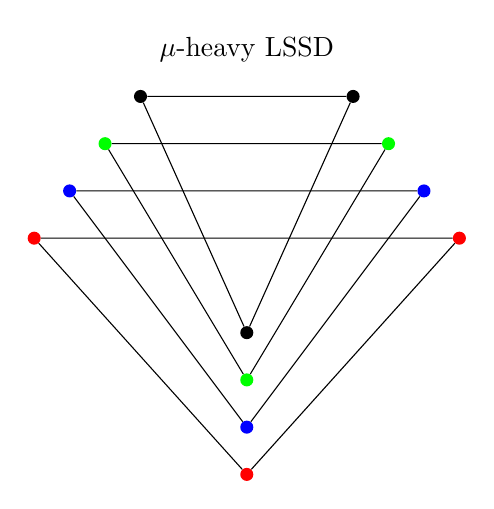
\begin{tikzpicture}[scale = .6,node distance=3cm,
thin,main node/.style={circle,fill=black,scale = .5}]
\node at (0,5) {$\mu$-heavy LSSD};
\def\x{1.5};
\node[main node,color = red] (11) at (-3*\x,1) {};
\node[main node,color = blue] (12) at (-2.5*\x,2) {};
\node[main node,color = green] (13) at (-2*\x,3) {};
\node[main node] (14) at (-1.5*\x,4) {};
\node[main node] (24) at (1.5*\x,4) {};
\node[main node,color = green] (23) at (2*\x,3) {};
\node[main node,color = blue] (22) at (2.5*\x,2) {};
\node[main node,color = red] (21) at (3*\x,1) {};
\node[main node] (34) at (0*\x,-1) {};
\node[main node,color = green] (33) at (0*\x,-2) {};
\node[main node,color = blue] (32) at (0*\x,-3) {};
\node[main node,color = red] (31) at (0*\x,-4) {};

\draw [-] (11) -- (21) -- (31) -- (11);
\draw [-] (12) -- (22) -- (32) -- (12);
\draw [-] (13) -- (23) -- (33) -- (13);
\draw [-] (14) -- (24) -- (34) -- (14);
\end{tikzpicture}\qquad
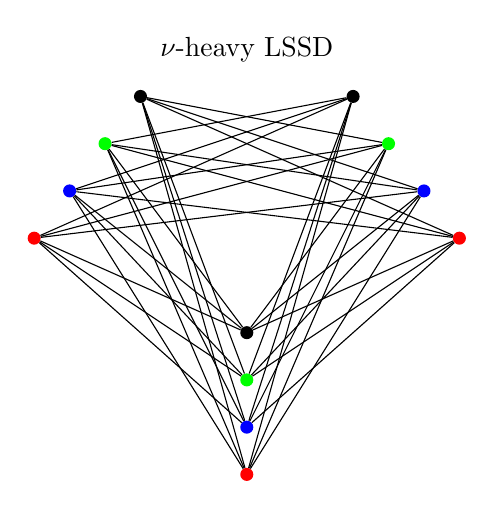
\begin{tikzpicture}[scale = .6,node distance=3cm,
thin,main node/.style={circle,fill=black,scale = .5}]
\node at (0,5) {$\nu$-heavy LSSD};
\def\x{1.5};
\node[main node,color = red] (11) at (-3*\x,1) {};
\node[main node,color = blue] (12) at (-2.5*\x,2) {};
\node[main node,color = green] (13) at (-2*\x,3) {};
\node[main node] (14) at (-1.5*\x,4) {};
\node[main node] (24) at (1.5*\x,4) {};
\node[main node,color = green] (23) at (2*\x,3) {};
\node[main node,color = blue] (22) at (2.5*\x,2) {};
\node[main node,color = red] (21) at (3*\x,1) {};
\node[main node] (34) at (0*\x,-1) {};
\node[main node,color = green] (33) at (0*\x,-2) {};
\node[main node,color = blue] (32) at (0*\x,-3) {};
\node[main node,color = red] (31) at (0*\x,-4) {};

\draw [-] (11) -- (22);
\draw [-] (11) -- (23);
\draw [-] (11) -- (24);
\draw [-] (11) -- (32);
\draw [-] (11) -- (33);
\draw [-] (11) -- (34);

\draw [-] (12) -- (21);
\draw [-] (12) -- (23);
\draw [-] (12) -- (24);
\draw [-] (12) -- (31);
\draw [-] (12) -- (33);
\draw [-] (12) -- (34);

\draw [-] (13) -- (32);
\draw [-] (13) -- (31);
\draw [-] (13) -- (34);
\draw [-] (13) -- (22);
\draw [-] (13) -- (21);
\draw [-] (13) -- (24);

\draw [-] (14) -- (22);
\draw [-] (14) -- (23);
\draw [-] (14) -- (21);
\draw [-] (14) -- (32);
\draw [-] (14) -- (33);
\draw [-] (14) -- (31);

\draw [-] (21) -- (32);
\draw [-] (21) -- (33);
\draw [-] (21) -- (34);
\draw [-] (22) -- (31);
\draw [-] (22) -- (33);
\draw [-] (22) -- (34);
\draw [-] (23) -- (32);
\draw [-] (23) -- (31);
\draw [-] (23) -- (34);
\draw [-] (24) -- (32);
\draw [-] (24) -- (33);
\draw [-] (24) -- (31);



\end{tikzpicture}\]
In this case the $\mu$-heavy LSSD has design parameters $(v,1,0)$, so we find that $s = \sqrt{k-\lambda} = 1$, $\nu = \frac{k(k-s)}{v} = 0$, and $\mu = \nu+s = 1$. We list the eigenmatrices and use these to further describe the LSSD:
\[\scalebox{.9}{$P = \left[\begin{array}{cccc}
1&w-1&v-1&(v-1)(w-1)\\
1&w-1&-1&-(w-1)\\
1&-1&-1&1\\
1&-1&v-1&1-v\\
\end{array}\right],\qquad Q = \left[\begin{array}{cccc}
1 & v-1 & (w-1)(v-1) & w-1\\
1 & v-1 & -(v-1) & -1\\
1 & -1 & 1-w & w-1\\
1 & -1 & 1 & -1\\
\end{array}\right]$}.\]
This means that our first idempotent is given by:
\[E_1 = (v-1)I+(v-1)A_1-A_2-A_3 = (vI-J)\otimes J.\]
If we scale this appropriately to obtain a Gram matrix of unit vectors, we find that $E_1$ is the Gram matrix of $w$ copies of the same simplex in $\mathbb{R}^v$. This can be seen as well from the fact that $Q_{01} = Q_{11}$ meaning that any simplex vector has inner product 1 with exactly one vector from each of the ``other" simplices, meaning the simplices are just copies of the same simplex. This explains why $w$ is unbounded as we can always copy the same simplex as many times as we would like. This also indicates why this example is not of interest to us as it is not giving $w$ distinct linked simplices.
\subsection{Cameron-Seidel scheme}\index{Cameron-Seidel Scheme}
\label{kerdock}
This construction is given originally by Goethals \cite{Goethals1976} in terms of Kerdock codes, though it was extensively studied by Cameron and Seidel. A restating of this concept is found in \cite{Bey2008}, where Bey and Kyureghyan frame the properties of Kerdock sets in terms of bent functions rather than quadratic forms. In addition, Kantor \cite{Kantor1982} showed that there are exponentially many non-isomorphic non-linear binary codes having Kerdock parameters.
\begin{definition}[\cite{Cameron1973}]
	Let $V=V(2m,2)$ be a $2m$-dimensional vector space over the field $\mathbb{F} = GF(2)$, ($m\geq 2$). A quadratic form on $V$ is a function $Q$ from $V$ to $\mathbb{F}$ with the properties
	\begin{itemize}
		\item[(i)] $Q(x_0) = 0$, where $x_0$ is the zero vector;
		\item[(ii)] The function $B = B(Q)$: $V\times V\rightarrow\mathbb{F}$ defined by
		\[B(x,y) = Q(x+y) + Q(x)+Q(y), \forall x,y\in V\]
		is bilinear.
	\end{itemize}
\end{definition}
We note that, over any field $\mathbb{F}$, the bilinear form corresponding to any quadratic form is symmetric $(B(x,y) = B(y,x))$. In the specific case of $\mathbb{F} = GF(2)$ however, this bilinear form is also alternating $(B(x,x) = 0)$. That is, for any $x\in V$, $B(x,x) = Q(x+x) + Q(x) + Q(x) = Q(2x) + 2Q(x) = 0$. Thus, within this context, we associate any quadratic form with an alternating bilinear form given by a square matrix with 0's on the main diagonal.

We now give a derivation of the Kerdock codes coming from quadratic forms. Let $Q_1,Q_2,\dots,Q_w$ be a set of $w$ quadratic forms on $\mathbb{Z}_2^n$ for which $Q_i+Q_j$ is a full rank quadratic form whenever $i\neq j$. Note that, through evaluation, each quadratic form gives us a vector $[Q_i(v)]_{v\in\mathbb{Z}^n_2}$ of length $2^n$. Let $\mathcal{Q}_1,\mathcal{Q}_2,\dots,\mathcal{Q}_w$ be cosets, $\mathcal{Q}_i = [Q_i(v)]_{v\in\mathbb{Z}_2^n}+\mathscr{R}(1,n)$, of the first order Reed Muller code (see \cite[Section 4.5]{vanLint1999}). For each $1\leq i\leq w$, define the shortening of $\mathcal{Q}_i$ as the set of vectors
\[V_i = \big\{\left[q(1),q(2),\dots,q\left(2^n-1\right)\right]\mid q(2^n) = 0\big\}_{q\in\mathcal{Q}_i}\]
where $q(j)$ denotes the $j^\text{th}$ entry of $q$. Since $\mathcal{Q}_i$ is closed under complements, we know that $\vert V_i\vert = \frac{1}{2}\vert\mathcal{Q}_i\vert = 2^{n}$. Further, any pair of vectors $v,w\in\bigcup_iV_i$ come from vectors $q_v,q_w\in\bigcup_i\mathcal{Q}_i$ with last entry $0$, so $wt(v\oplus w) = wt(q_v\oplus q_w)$ where $wt(x)$, the Hamming weight of the binary tuple $x$, is equal to the number of non-zero entries. Finally, for each $i$, construct the set of vectors
\[X_i = \left\{\frac{1}{\sqrt{2^n-1}}\left(2v-\mathbbm{1}\right)\vert v\in V_i\right\}.\]
We claim $\left\{X_i\right\}_{i=1..w}$ is a set of linked simplices. To verify this, fix $1\leq i<j\leq w$ and let $x_i,y_i\in X_i$ and $z_j\in X_j$ with corresponding coset vectors $q_x,q_y,$ and $q_z$ respectively. Then,
\[\begin{aligned}
\left<x_i,x_i\right> &= \frac{1}{2^n-1}\left((wt(x_i)+(-1)^2(2^{n}-1-wt(x_i))\right)=1
\end{aligned}\]
giving that every vector in $\bigcup_iX_i$ is a unit vector. Next,
\[\begin{aligned}
\left<x_i,y_i\right> &= \frac{1}{2^n-1}\left((2^n-1)-2wt(q_x\oplus q_y)\right)=-\frac{1}{2^n-1}
\end{aligned}\]
giving us that $X_i$ forms a regular simplex. Finally,
\[\begin{aligned}
\left<x_i,z_j\right> &= \frac{1}{2^n-1}\left((2^n-1)-2wt(q_x\oplus q_w)\right).
\end{aligned}\]
Since $wt(q_x\oplus q_z)\in \left\{2^{n-1}\pm2^{r-1}\right\}$ we have that
\[\left<x_i,w_j\right> = \begin{cases}
\frac{2^{r}-1}{2^{n}-1} & wt(q_x\oplus q_w) = 2^{n-1}-2^{r-1}\\
-\frac{2^r+1}{2^n-1} & wt(q_x\oplus q_w) = 2^{n-1}+2^{r-1}\\
\end{cases}\]
meaning there are two possible angles between simplices.\par
Therefore we can build a LSSD with $w$ fibers whenever we have $w$ quadratic forms whose pairwise sums are full rank. We represent each quadratic form as the $n\times n$ matrix giving the corresponding alternating bilinear form. Then, any two of these matrices must differ in the first row in order for their difference to be full rank. This means $w\leq2^{n-1}$ as there are only $2^{n-1}$ possible choices for the first row. This upper bound is achievable whenever $n$ is even \cite{Cameron1973}. Below we give an example when $n = 4$ where $Q_i$ is the alternating bilinear form corresponding to the $i^{\text{th}}$ quadratic form.
\setlength{\arraycolsep}{2.5pt}
\[\begin{aligned}
Q_1 &= \left[\begin{array}{cccc}
0 & 0 & 0 & 0\\
0 & 0 & 0 & 0\\
0 & 0 & 0 & 0\\
0 & 0 & 0 & 0\\
\end{array}\right],\quad Q_2 = \left[\begin{array}{cccc}
0 & 1 & 0 & 0\\
1 & 0 & 0 & 0\\
0 & 0 & 0 & 1\\
0 & 0 & 1 & 0\\
\end{array}\right],\quad Q_3 = \left[\begin{array}{cccc}
0 & 0 & 1 & 0\\
0 & 0 & 0 & 1\\
1 & 0 & 0 & 1\\
0 & 1 & 1 & 0\\
\end{array}\right],\quad
Q_4 = \left[\begin{array}{cccc}
0 & 1 & 1 & 0\\
1 & 0 & 1 & 1\\
1 & 1 & 0 & 0\\
0 & 1 & 0 & 0\\
\end{array}\right],
\\
Q_5 &= \left[\begin{array}{cccc}
0 & 0 & 0 & 1\\
0 & 0 & 1 & 1\\
0 & 1 & 0 & 1\\
1 & 1 & 1 & 0\\
\end{array}\right],\quad
Q_6 = \left[\begin{array}{cccc}
0 & 1 & 0 & 1\\
1 & 0 & 1 & 0\\
0 & 1 & 0 & 0\\
1 & 0 & 0 & 0\\
\end{array}\right],\quad Q_7 = \left[\begin{array}{cccc}
0 & 0 & 1 & 1\\
0 & 0 & 1 & 0\\
1 & 1 & 0 & 1\\
1 & 0 & 1 & 0\\
\end{array}\right],\quad Q_8 =\left[\begin{array}{cccc}
0 & 1 & 1 & 1\\
1 & 0 & 0 & 1\\
1 & 0 & 0 & 0\\
1 & 1 & 0 & 0\\
\end{array}\right].\\
\end{aligned}\]
It is straightforward to form the characteristic vectors $[Q_i(v)]_v$. Below we display $[Q_2(v)]_v$ and $[Q_8(v)]_v$:
\[\begin{aligned}
\left[Q_2(v)\right]_v &= \left[\begin{array}{cccccccccccccccc}0 & 0 & 0 & 1 & 0 & 0 & 0 & 1 & 0 & 0 & 0 & 1 & 1 & 1 & 1 & 0\end{array}\right],\\
[Q_8(v)]_v &= \left[\begin{array}{cccccccccccccccc}0 & 0 & 0 & 1 & 0 & 1 & 0 & 0 & 0 & 1 & 1 & 1 & 0 & 0 & 1 & 0\end{array}\right].\\
\end{aligned}\]
Each of these binary vectors of length 16 is a codeword in the second-order Reed-Muller code $\scR(2,4)$, thus each codeword then determines a coset of $\scR(1,4)$ inside $\scR(2,4)$. The coset corresponding to $Q_2(v)$ is given below as the set of rows of the matrix. To improve readability, $+$ denotes a $1$ and an empty space denotes a $0$.
\[[Q_2(v)]_v+\mathscr{R}(1,4) =\setlength{\arraycolsep}{.8pt}{\fontsize{5}{6}\selectfont\left[\begin{array}{cccccccccccccccc}
	&  &  & + &  &  &  & + &  &  &  & + & + & + & + & \\
	+ & + & + &  & + & + & + &  & + & + & + &  &  &  &  & +\\
	& + &  &  &  & + &  &  &  & + &  &  & + &  & + & +\\
	+ &  & + & + & + &  & + & + & + &  & + & + &  & + &  & \\
	+ & + &  & + & + & + &  & + & + & + &  & + &  &  & + & \\
	&  & + &  &  &  & + &  &  &  & + &  & + & + &  & +\\
	+ &  &  &  & + &  &  &  & + &  &  &  &  & + & + & +\\
	& + & + & + &  & + & + & + &  & + & + & + & + &  &  & \\
	+ & + & + &  &  &  &  & + & + & + & + &  & + & + & + & \\
	&  &  & + & + & + & + &  &  &  &  & + &  &  &  & +\\
	+ &  & + & + &  & + &  &  & + &  & + & + & + &  & + & +\\
	& + &  &  & + &  & + & + &  & + &  &  &  & + &  & \\
	&  & + &  & + & + &  & + &  &  & + &  &  &  & + & \\
	+ & + &  & + &  &  & + &  & + & + &  & + & + & + &  & +\\
	& + & + & + & + &  &  &  &  & + & + & + &  & + & + & +\\
	+ &  &  &  &  & + & + & + & + &  &  &  & + &  &  & \\
	+ & + & + &  & + & + & + &  &  &  &  & + & + & + & + & \\
	&  &  & + &  &  &  & + & + & + & + &  &  &  &  & +\\
	+ &  & + & + & + &  & + & + &  & + &  &  & + &  & + & +\\
	& + &  &  &  & + &  &  & + &  & + & + &  & + &  & \\
	&  & + &  &  &  & + &  & + & + &  & + &  &  & + & \\
	+ & + &  & + & + & + &  & + &  &  & + &  & + & + &  & +\\
	& + & + & + &  & + & + & + & + &  &  &  &  & + & + & +\\
	+ &  &  &  & + &  &  &  &  & + & + & + & + &  &  & \\
	&  &  & + & + & + & + &  & + & + & + &  & + & + & + & \\
	+ & + & + &  &  &  &  & + &  &  &  & + &  &  &  & +\\
	& + &  &  & + &  & + & + & + &  & + & + & + &  & + & +\\
	+ &  & + & + &  & + &  &  &  & + &  &  &  & + &  & \\
	+ & + &  & + &  &  & + &  &  &  & + &  &  &  & + & \\
	&  & + &  & + & + &  & + & + & + &  & + & + & + &  & +\\
	+ &  &  &  &  & + & + & + &  & + & + & + &  & + & + & +\\
	& + & + & + & + &  &  &  & + &  &  &  & + &  &  & \\
	\end{array}\right]}.\]
To form our regular simplex we now choose all vectors with 0 in the last coordinate, discard the last entry, replace every 0 with a $-1$ (abbreviated to $-$), and then scale by $\frac{1}{\sqrt{15}}$ giving us the vectors (given by rows):
\[\begin{aligned}
X_2 = \frac{1}{\sqrt{15}}\setlength{\arraycolsep}{.8pt}{\fontsize{5}{6}\selectfont\left[\begin{array}{rrrrrrrrrrrrrrrr}
	- & - & - & + & - & - & - & + & - & - & - & + & + & + & + \\
	+ & - & + & + & + & - & + & + & + & - & + & + & - & + & - \\
	+ & + & - & + & + & + & - & + & + & + & - & + & - & - & + \\
	- & + & + & + & - & + & + & + & - & + & + & + & + & - & - \\
	+ & + & + & - & - & - & - & + & + & + & + & - & + & + & + \\
	- & + & - & - & + & - & + & + & - & + & - & - & - & + & - \\
	- & - & + & - & + & + & - & + & - & - & + & - & - & - & + \\
	+ & - & - & - & - & + & + & + & + & - & - & - & + & - & - \\
	+ & + & + & - & + & + & + & - & - & - & - & + & + & + & + \\
	- & + & - & - & - & + & - & - & + & - & + & + & - & + & - \\
	- & - & + & - & - & - & + & - & + & + & - & + & - & - & + \\
	+ & - & - & - & + & - & - & - & - & + & + & + & + & - & - \\
	- & - & - & + & + & + & + & - & + & + & + & - & + & + & + \\
	+ & - & + & + & - & + & - & - & - & + & - & - & - & + & - \\
	+ & + & - & + & - & - & + & - & - & - & + & - & - & - & + \\
	- & + & + & + & + & - & - & - & + & - & - & - & + & - & - \\
	\end{array}\right]}.
\end{aligned}\]
Likewise each $[Q_j(v)]_v$ gives us a coset of size 32, which in turn is transformed to a regular simplex $X_j$ of sixteen vectors in $\mathbb{R}^{15}$ in this manner.
\subsubsection*{Symmetric design parameters}
The design parameters of this scheme are $\left(2^{2r},2^{r-1}\left(2^{r}+1\right),2^{r-1}\left(2^{r-1}+1\right)\right)$. Using these, we have: $s = 2^{r-1}$, $\nu = 2^{r-2}\left(2^r+1\right)$,  and $\mu=2^{r-2}\left(2^r+3\right)$.
\subsubsection*{Intersection numbers}
Noting that $p_{ij}^k = p_{ji}^k$, we list the unique intersection numbers while omitting the trivial $p_{0i}^j$ parameters. Note that each $p^{j}_{ik}$ is scaled by a constant based on $i$ and $k$ given in the top row of our table.
\[\scalebox{.9}{$\begin{array}{c|ccc|cc|c}
j & \bigslant{p^{j}_{11}}{2^{r-2}}			& \bigslant{p^{j}_{12}}{2^{r-1}} 			& \bigslant{p^{j}_{13}}{2^{r-2}} & p^{j}_{22} & \bigslant{p^{j}_{23}}{2^{r-1}} & \bigslant{p^{j}_{33}}{2^{r-2}}\\\hline
0 & \left(2^{r+1}+2\right)(w-1)	& 0 							& 0 					& 2^{2r}-1	& 0   							& (2^{r+1}-2)(w-1)\\
1 & \left(2^r+3\right)(w-2)		& \left(2^{r}+1\right)-2^{1-r}	& (2^r-1)(w-2) 			& 0   		& \left(2^r-1\right)   			& \left(2^{r-2}-1\right)(w-2)\\
2 & \left(2^{r}+2\right)(w-1)	& 0 							& 2^{r}(w-1)			& 2^{2r}-2 	& 0 							& (2^{r}-2)(w-1)\\
3 & \left(2^r+1\right)(w-2) 	& 2^{r}+1						& (2^r+1)(w-2) 			& 0   		&\left(2^{r}-1\right)-1 		& \left(2^{r-2}-3\right)(w-2)\\
\end{array}$}\]
\subsubsection*{Krein parameters}
As with the intersection numbers, we recall that $q_{ij}^k = q_{ji}^k$ and list each unique Krein parameter omitting the trivial $q_{0i}^j$ parameters. No scaling is done here.
\[\begin{array}{c|ccc|cc|c}
j & q^{j}_{11}			& q^{j}_{12}							& q^{j}_{13}	& q^{j}_{22} 						& q^{j}_{23} 	& q^{j}_{33}\\\hline
0 & 2^{2r}-1			& 0										& 0 			& (w-1)(2^{2r}-1)								& 0  			& w-1\\
1 & \frac{2^{2r}}{w}-2	& 2^{2r}\left(\frac{w-1}{w}\right)		& 0 			& \frac{2^{2r}(w-1)^2}{w}-2(w-1)	& w-1			& 0\\
2 & \frac{2^{2r}}{w}	& 2^{2r}\left(\frac{w-1}{w}\right)-2	& 1				& \frac{2^{2r}(w-1)^2}{w}+2(w-2)	& w-2			& 0\\
3 & 0 					& 2^{2r}-1								& 0 			& (w-2)(2^{2r}-1)								& 0  			& w-2\\
\end{array}\]

\section{New examples with \texorpdfstring{$v\neq 2^m$}{v not equal to a power of 2}}
\label{LSSDMUBs}
Recall from Section $\ref{bases}$ that we found the Gram matrix for a set of bases by adding the first two idempotents of our scheme, giving us
\begin{equation}\label{MubGram}M = w(E_0+E_1) = \left(A_0+\frac{v-k+\sqrt{k-\lambda}}{v\sqrt{k-\lambda}}A_1-\frac{k-\sqrt{k-\lambda}}{v\sqrt{k-\lambda}}A_3\right)\end{equation}
where $k$ is the block size of the $\mu$-heavy LSSD. If $\frac{v-k+\sqrt{k-\lambda}}{v\sqrt{k-\lambda}}$ and $-\frac{k-\sqrt{k-\lambda}}{v\sqrt{k-\lambda}}$ have the same absolute value, then $M$ is the Gram matrix for a set of $w$ mutually unbiased bases in $\mathbb{R}^v$. This will only occur when
\[\begin{aligned}v-2k&=-2\sqrt{k-\lambda}.\\
\end{aligned}\]
This means our LSSD must be optimistic, leading to the following lemma:
\begin{lem}
	\label{twoside}
	Let $\mathbb{A}$ be the Bose-Mesner algebra of an optimistic $LSSD(v,k,\lambda;w)$ with $Q$-polynomial ordering $E_0,E_1,E_2,E_3$ of its primitive idempotents. If $\vert v-2k\vert = 2\sqrt{k-\lambda}$ then $w(E_0+E_1)$ is the Gram matrix of a set of $w$ real MUBs in dimension $v$.\qed
\end{lem}
It is important to note here that there exist pessimistic LSSDs such that $v-2k = 2\sqrt{k-\lambda}$. One such example is a specific case of the degenerate design parameters in Section \ref{degenerate} given by $(v,k,\lambda)=(4,1,0)$ with the graph $\Gamma_1$ displayed below.
\[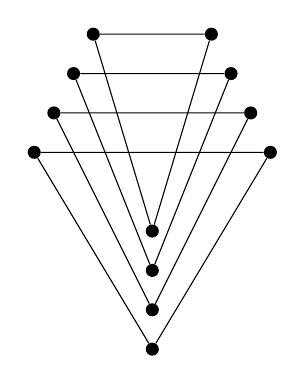
\begin{tikzpicture}[scale = .5,node distance=2cm,
thin,main node/.style={circle,fill=black,scale = .5}]

\node[main node] (11) at (-3,1) {};
\node[main node] (12) at (-2.5,2) {};
\node[main node] (13) at (-2,3) {};
\node[main node] (14) at (-1.5,4) {};
\node[main node] (24) at (1.5,4) {};
\node[main node] (23) at (2,3) {};
\node[main node] (22) at (2.5,2) {};
\node[main node] (21) at (3,1) {};
\node[main node] (34) at (0,-1) {};
\node[main node] (33) at (0,-2) {};
\node[main node] (32) at (0,-3) {};
\node[main node] (31) at (0,-4) {};

\draw [-] (11) -- (21) -- (31) -- (11);
\draw [-] (12) -- (22) -- (32) -- (12);
\draw [-] (13) -- (23) -- (33) -- (13);
\draw [-] (14) -- (24) -- (34) -- (14);
\end{tikzpicture}\]
We can easily see that $v-2k = 2 = 2\sqrt{k-\lambda}$. However, the sum of the first two eigenspaces gives
\[M = 3(E_0 + E_1) =\frac{1}{3}A_0 -\frac{1}{4}A_1\]
which is not the Gram matrix of a set of MUBs. In fact, any Menon parameter set with $v/4$ odd will satisfy $\vert v-2k\vert = 2\sqrt{k-\lambda}$ yet none of these will produce MUBs. Thus our restriction to optimistic LSSDs is required and we cannot say that any LSSD satisfying $\vert v-2k\vert = 2\sqrt{k-\lambda}$ will give us MUBs using this construction. Conversely, the existence of $w$ MUBs in $\mathbb{R}^v$ does not guarantee the existence of an optimistic $LSSD(v,k,\lambda;w)$; consider 3 MUBs in $\mathbb{R}^4$.
\subsection{Restrictions on the design parameters}
In this section, we show that $\vert v-2k\vert = 2\sqrt{k-\lambda}$ implies $(v,k,\lambda)$ are Menon design parameters. In the case of optimistic LSSDs, we also show $v/4$ is even. We now take a closer look at our restriction $v-2k = -2\sqrt{k-\lambda}$. First note we can square both sides to get
\[\begin{aligned}
4(k-\lambda)&=v^2-4k(v-k).
\end{aligned}\]
Using \eqref{sym:2}, this gives $v=4(k-\lambda)$ where we apply \eqref{sym:1} to get
\[k^2+k+\lambda=4\lambda(k-\lambda).\]
Solving this for $k$ gives $k=\frac{4\lambda+1}{2}\pm\frac{\sqrt{4\lambda+1}}{2}$ requiring $\frac{1}{2}\pm\frac{1}{2}\sqrt{4\lambda+1}$ to be an integer. Therefore $\sqrt{4\lambda+1}$ must be an odd integer. Assume $4\lambda+1 = (2u-1)^2$ for some positive integer $u$. Then $\lambda = u^2-u$ and
\[\begin{aligned}
k&=2u^2-(2\mp 1)u+\left(\frac{1\mp1}{2}\right).\\
\end{aligned}\]
If we re-parameterize the second family to avoid the trivial $(0,0,0)$ design when $u=1$, we get the complementary families:
\[\begin{aligned}
\lambda &= (u-1)u\qquad\qquad &\lambda^\prime &= (u+1)u\\
k&=(2u-1)u\qquad \text{and}\qquad&k^\prime &= (2u+1)u\\
v&= 4u^2\qquad \qquad&v^\prime &= 4u^2.
\end{aligned}\]
If we restrict to an optimistic LSSD, we must use the second family for our $\mu$-heavy LSSD $\Gamma$. From \eqref{mu-nu}, we find
\[\begin{aligned}
s=\sqrt{k-\lambda}=u,\qquad\nu =\frac{k(k-s)}{v}=u^2+\frac{u}{2},\qquad\mu=\nu+s=u^2+\frac{3}{2}u.
\end{aligned}\]
This forces $\nu$ (and $\mu$) to be integral if and only if $u$ is even, resulting in the following theorem
\begin{thm}
	\label{MubLssdrestrictions}
	Let $\Gamma$ be an optimistic $LSSD(v,k,\lambda;w)$. If $v-2k = -2\sqrt{k-\lambda}$ then $(v,k,\lambda)$ are \emph{Menon design parameters}\index{Menon parameters}. That is,
	\begin{enumerate}[label=$(\roman*)$]
		\item $v = 4u^2$
		\item $k = 2u^2+u$
		\item $\lambda = u^2+u$
		\item $w\leq 2u^2$
	\end{enumerate}
	Further, if $u$ is odd, then $w = 2$.
\end{thm}
\begin{proof}
	Statements \emph{(i) -- (iii)} as well as our restriction when $u$ is odd follow directly from above. Conclusion \emph{(iv)} follows from \eqref{Noda}.
\end{proof}
The upper bound for $w$ is achieved whenever $u$ is a power of two using the Cameron-Seidel scheme. In light of this family and the condition that $w=2$ whenever $v/4$ is odd, one might ask if $w$ is bounded as a function of the highest power of $2$ dividing $v$. We will show later that this is not true by constructing examples with $w$ as large as we like and $v/16$ odd.
\subsection{Mutually unbiased Hadamard matrices}
In this section, we establish an equivalence between LSSDs with design parameters as in Theorem \ref{MubLssdrestrictions} with sets of regular unbiased Hadamard matrices (see \cite{Kharaghani2010} for more detailed information on unbiased Hadamard matrices). Van Dam et al.\ \cite[p.~1423]{Davis2014} briefly mention this connection citing constructions of unbiased regular Hadamard matrices by Holzmann, Kharaghani, and Orrick \cite{Kharaghani2010} using mutually orthogonal latin squares. In this section, we describe the connection between unbiased regular Hadamard matrices and LSSDs in full, using Theorem \ref{twoside}. A real Hadamard matrix\index{Hadamard matrix!real} of order $v$ is a $v\times v$ matrix $H$ with entries $\pm 1$ such that $HH^T = vI$. $H$ is a \textit{regular Hadamard matrix}\index{Hadamard matrix!regular} if $HJ = JH = cJ$ for some constant $c$; one easily verifies that $c = \sqrt{v}$. Two Hadamard matrices $H_1$ and $H_2$ are \textit{unbiased}\index{Hadamard matrix!unbiased} if $\frac{1}{\sqrt{v}}H_1H_2^T$ is itself a Hadamard matrix. Finally, a set of Hadamard matrix matrices are mutually unbiased if each pair is unbiased. Using these definitions, consider the following:
\begin{thm}
	\label{LSSDtoHad}
	Let $\Gamma$ be an optimistic $LSSD(v,k,\lambda;w)$. If $\vert v-2k\vert = 2\sqrt{k-\lambda}$, then there exists a set of $w-1$ real mutually unbiased regular Hadamard matrices of order $v$.
\end{thm}
\begin{proof}
	Let $(X,\mathcal{R})$ be the association scheme arising from $\Gamma$ with Bose-Mesner algebra $\mathbb{A}$. Let $\left\{E_0,E_1,E_2,E_3\right\}$ be the set of idempotents under the natural $Q$-polynomial ordering. From Lemma \ref{twoside}, $G = w(E_0+E_1)$ is the Gram matrix of a set of $w$ MUBs in $\mathbb{R}^v$. Let the $w$ MUBs be given by the columns of the $w$ orthogonal matrices $\left\{M_1,\dots,M_w\right\}$ and without loss of generality assume $M_1 = I$. Then any column from another $M_i$ $(i\neq 1)$ must have entries $\pm \frac{1}{\sqrt{v}}$. For $1<i\leq w$, let $H_i = \sqrt{v}M_i$. First note that $H_iH_i^T = vM_iM_i^T = vI$, therefore for each $1<i\leq w$, $H_i$ is a Hadamard matrix. Now consider that the first $v$ rows of $G$ will have the block form
	$\left[\begin{array}{ccccc}
	I & M_2 & M_3 & \dots & M_{w}\\
	\end{array}\right].$
	However from \eqref{MubGram}, we have that the positive (resp., negative) entries of $M_i$ represent adjacency between vertices in the first and $i^\text{th}$ fibers of the $\mu$-heavy (resp., $\nu$-heavy) LSSD. Since each vertex in the first fiber must be adjacent to $k$ vertices in the $i^\text{th}$ fiber in the $\mu$-heavy LSSD, each row of $M_i$ must have $k$ positive entries and $v-k$ negative entries. Similarly, each vertex in the $i^\text{th}$ fiber is adjacent to $k$ vertices in the first fiber in the $\mu$-heavy LSSD, thus each column of $M_i$ has $k$ positive entries and $v-k$ negative entries. Therefore each $H_i$ must be regular. Now define $\binom{w}{2}$ matrices $M_{i,j}$ where $M_{i,j}$ is the orthogonal matrix representing basis $j$ when basis $i$ is taken to be the standard basis (so $M_{1,j} = M_j$). Then we repeat all previous arguments to show that $G$ has the block form:
	\[G = \left[\begin{array}{ccccccc}
	I & M_{1,2} & \dots & M_{1,w}\\
	M_{2,1} & I & \dots & M_{2,w}\\
	\vdots & \vdots  & \ddots & \vdots\\
	M_{w,1} & M_{w,2} & \dots & I\\
	\end{array}\right]\]
	where $\sqrt{v}M_{i,j}$ is a Hadamard matrix for all $1\leq i\neq j\leq w$. Now consider a second association scheme $(X',\cR')$ arising from the subgraph of $\Gamma$ induced on three distinct fibers $X_i$, $X_j$, and $X_k$. The matrix $G^\prime = w(E_0^\prime + E_1^\prime)$ will have the form:
	\[G^\prime = \left[\begin{array}{ccccccc}
	I & M_{i,j} & M_{i,k}\\
	M_{j,i} & I  & M_{j,k}\\
	M_{k,i} & M_{k,j} & I\\
	\end{array}\right].\]
	Noting that $G^2 = wG$, the block in the $(1,2)$ block of $G^2$ gives us that
	\[2M_{i,j} + M_{i,k}M_{k,j} = 3M_{i,j},\qquad \text{ or equivalently } \qquad M_{i,k}M_{k,j} = M_{i,j}.\]
	Therefore, if we return to the original $LSSD$ and define $H_{i,j} = \sqrt{v}M_{i,j}$, we find that $\frac{1}{\sqrt{v}}H_i^TH_j = H_{i,j}$. It follows that the set $\left\{H_2,\dots,H_w\right\}$ is a set of $w-1$ regular mutually unbiased Hadamard matrices.
\end{proof}
We now show the converse:
\begin{thm}
	Assume $w>2$. Let $\left\{H_2,\dots,H_w\right\}$ be $w-1$ regular unbiased Hadamard matrices of order $v$. Then there exists an optimistic $LSSD(v,k,\lambda;w)$.
\end{thm}
\begin{proof}
	Assume without loss of generality that the row sum of each of our Hadamard matrices is positive. Define vectors $x_{i,j}$ for $2\leq i\leq w$ and $1\leq j\leq v$ such that $x_{i,j}$ is the $j^\text{th}$ column of $H_i-\frac{1}{\sqrt{v}}J$. Let $x_{1,j}$ be the $j^\text{th}$ column of $\sqrt{v}I-\frac{1}{\sqrt{v}}{J}$. Note that for all $1\leq i\leq w$, $\vnorm{x_{i,j}} = v-1$. Then, for all $i,j$, let $\hat{x}_{i,j} = \frac{x_{i,j}}{\sqrt{v-1}}$. Letting $X_i = \left\{\hat{x}_{i,1},\dots,\hat{x}_{i,v}\right\}$, we claim that $\left\{X_1,\dots, X_w\right\}$ is a set of linked simplices. To show this, fix $j\neq k$, $i\neq i'$ and consider the following four inner products:
	\begin{align}
	\label{had:1}\left<\hat{x}_{1,j},\hat{x}_{1,k}\right> &= \frac{1}{v-1}\left[vI-J\right]_{j,k} = -\frac{1}{v-1},\\
	\label{had:2}\left<\hat{x}_{i,j},\hat{x}_{i,k}\right> &=\frac{1}{v-1}\left[H_iH_i^T -J\right]_{j,k} = -\frac{1}{v-1},\\
	\label{had:3}\left<\hat{x}_{1,j},\hat{x}_{i,k}\right> &=\frac{\sqrt{v}}{v-1}\left[H_i^T-\frac{1}{\sqrt{v}}J\right]_{j,k},\\
	\label{had:4}\left<\hat{x}_{i,j},\hat{x}_{i',k}\right> &=\frac{\sqrt{v}}{v-1}\left[\frac{1}{\sqrt{v}}H_iH_{i^\prime}^T -\frac{1}{\sqrt{v}}J\right]_{j,k}.
	\end{align}
	\eqref{had:1} and \eqref{had:2} give us the inner products within each $X_i$. Since $\frac{1}{\sqrt{v}}H_iH_{i^\prime}^T$ is a Hadamard matrix, \eqref{had:3} and \eqref{had:4} tell us that inner products between sets $X_i$ and $X_{i^\prime}$ take values of $\frac{\pm\sqrt{v}-1}{v-1}$. Finally note that the all ones vector is orthogonal to all $\hat{x}_{i,j}$, implying $\left\{X_1,\dots,X_w\right\}$ is a set of $w$ simplices in $\mathbb{R}^{v-1}$ such that inner products between simplices can take only two possible values. Finally consider that the possible inner products are $\frac{\sqrt{v}}{v-1}\left(\pm 1 - \frac{1}{\sqrt{v}}\right)$. This tells us that $\vert \gamma\vert <\vert \delta\vert$ where $\gamma$ is the positive inner product and $\delta$ is the negative. Since the centroid of any simplex is the origin, we must have more positive inner products between simplices than negative, telling us our $LSSD$ is optimistic.
\end{proof}
This provides us with the following theorem
\lssdhadequiv\vspace{-9mm}\qed
%\begin{thm}
%	\label{equiv}
%	An optimistic $LSSD(v,k,\lambda;w)$ with $\vert v-2k\vert = 2\sqrt{k-\lambda}$ exists if and only if there exists a set of $w-1$ regular unbiased Hadamard matrices with order $v$.\qed
%\end{thm}
\subsection{Constructing LSSDs from real MUBs}
Using the results from the last section and the close relation between MUBs and Hadamard matrices, we wish to build new LSSDs. From Theorem \ref{equiv} and Theorem \ref{MubLssdrestrictions}, we are only going to find optimistic LSSDs with Menon design parameters. The Cameron-Seidel scheme is a construction for $w = 2u^2$ whenever $u$ is a power of 2 (see Section \ref{kerdock}). We skip this case and instead look for constructions where $u$ (and equivalently $v$) is not necessarily a power of 2.
\subsubsection{Wocjan and Beth construction}
Wocjan and Beth in \cite{Wocjan2005} detail a way to create MUBs from MOLS. They take a set of $t$ MOLS with side length $d$ and create $t+2$ MUBs in dimension $d^2$. The process is to convert the MOLS into an orthogonal array with $d^2$ rows. They then expand the array by replacing each column with $d$ columns given by the characteristic vector of each symbol in that column. Finally, they extend this matrix by replacing each 1 in the array with a row from a Hadamard matrix and each 0 by an appropriate length vector of 0s. The result is that the $d$ columns arising from each original column are orthogonal to each other. We will focus on the case where the resultant MUBs produce regular Hadamard matrices as scalar multiples of the mixed Gram matrices between any pair of fibers.\par
For our purposes, an orthogonal array of size $(n^2\times N)$ has entries from the set $\left\{1,\dots, n\right\}$ and any two columns contain each ordered pair exactly once. Let $O$ be an orthogonal array of size $n^2\times N$, let $C^i$ denote the $i^{th}$ column of $O$ with entries $C^i_h$ ($1\leq h\leq n^2$). We may uniquely express
\[C^i = \sum_{j=1}^n jB^{i,j} \]
where each $B^{i,j}$ is a 01-vector of length $n^2$. As each symbol $j$ appears in each column $C^i$ exactly $n$ times, $B^{i,j}$ will have $n$ 1s and $n^2-n$ 0s. Let $H$ be a Hadamard matrix matrix of order $n$. For $1\leq l\leq n$ define a matrix $M^{i,j,l}$ as follows: for $1\leq h\leq n$, we replace the $h^\text{th}$ 1, counting from the top, in $B^{i,j}$ with the $H_{h,l}$. This produces $n^2N$ columns each with $n^2$ entries $M_h^{i,j,l}\in\left\{0,1,-1\right\}$.\par
The fact that $H^TH = nI$ together with $B^{i,j}\circ B^{i,j^\prime} = 0$ for $j\neq j^\prime$ give us that $\mathcal{B}_i = \left\{M^{i,1,1},\dots,M^{i,n,n}\right\}$ is an orthogonal basis for each $i=1,\dots,N$. Each vector in these bases has squared norm $n$. For $i\neq i'$, $C^i$ and $C^{i'}$ denote distinct columns in our orthogonal array implying, for any $j$ and $j'$ (not necessarily distinct), $B^{i,j}\circ B^{i',j'}$ has one non-zero entry. Then $M^{i,j,l}\circ M^{i',j',l'}$ also has one non-zero entry giving
\begin{equation}\left<M^{i,j,l},M^{i',j',l'}\right>=M^{i,j,l}_hM^{i',j',l'}_h=\pm 1\\
\end{equation}
where $O_{h,i} = j$ and $O_{h,i'} = j'$. This tells us the bases $\mathcal{B}_1,\dots,\mathcal{B}_s$ produced by Wocjan and Beth are pairwise unbiased.\par
We now show that if $H$ is regular, then the resulting unbiased Hadamard matrices are regular (see proof of Theorem \ref{LSSDtoHad} for the construction of these Hadamard matrices). For each Hadamard matrix, the row sum is the sum of inner products between a column $M^{i,j,l}$ of one basis with the set of $n^2$ columns $M^{i',j',l'}$ ($i\neq i'$, $1\leq j',l'\leq n)$ of the second basis used in its construction. We first sum $\left<M^{i,j,l},M^{i',j',l'}\right>$ over $l'$ to get
\begin{equation*}
\sum_{l'} \left<M^{i,j,l},M^{i',j',l'}\right>=M^{i,j,l}_h\left(\sum_{l'}M^{i',j',l'}_h\right)=pM^{i,j,l}_h
\end{equation*}
where $p$ is the row sum of our Hadamard matrix $H$. We then sum this result over $j'$, noting that $h$ was chosen so that $O_{h,i} = j$ and $O_{h,i'} = j'$, meaning it depends on $j'$. As this sum will include every non-zero entry in $M^{i,j,l}$ exactly once, we know
\begin{equation}
\label{rowsum}
\sum_{j'}\sum_{l'}\left<M^{i,j,l},M^{i',j',l'}\right> =\sum_{j'}pM^{i,j,l}_{h}=p\sum_{j'}H_{j',l}=p^2.
\end{equation}
Then the sum of any row of the Hadamard matrix built from $M^{i,j,l}$ and $M^{i',j',l'}$ ($i\neq i'$) will be $p^2$. Further, we showed in Theorem \ref{LSSDtoHad} that these Hadamard matrices are unbiased. Noting that $n = 4t^2$ for some $t$, Theorem \ref{equiv} tells us that the resultant LSSD will be an optimistic $LSSD(16t^4,k,\lambda;N)$. This leads to our final theorem.
\buildinghad
%\begin{thm}[{cf.\cite[Thm~13]{Kharaghani2010}}]
%	\label{newLSSD}
%	Given a regular Hadamard matrix of order $s$ and an orthogonal array of size $s^2\times N$,
%	\begin{itemize}
%		\item There exists $N-1$ regular unbiased Hadamard matrices of order $s^2$.
%		\item There exists a $LSSD$ with $v=s^2$ and $w=N$.\qed
%	\end{itemize}
%\end{thm}
The following theorem is due to Beth \cite{Beth1983} and will be used to show the number of fibers is unbounded as $v$ increases.
\begin{thm}\cite{Beth1983}\label{beth}
	Let $N(n)$ be the maximum size of a set of mutually orthogonal latin squares of side $n$. Then, for $n$ sufficiently large, $N(n)\geq n^\frac{1}{14.8}$.
\end{thm}
\asymplssd
%\begin{cor}
%	\label{asymptotics}
%	For sufficiently large $s$, if there exists a regular Hadamard matrix of order $s$, then there exists a $LSSD(s^2,k,\lambda; w)$ with $w \geq s^\frac{1}{14.8}$.
%\end{cor}
\begin{proof}
	Using Theorem \ref{beth}, we know that for sufficiently large $n$, we may find a set of mutually orthogonal latin squares of side $n$ with at least $n^\frac{1}{14.8}$ squares. However, given $t$ mutually orthogonal latin squares of side $n$, we may build an orthogonal array with $n+2$ columns with $n$ symbols. This is achieved by indexing the rows of our orthogonal array by the $n^2$ positions in a latin square. The first and second columns of the orthgonal array denote the row and column (resp.) of the position within the latin square. Each remaining column corresponds to one of the mutually orthogonal latin squares where the symbols in each position generate the column. Thus, as long as we may find a regular Hadamard matrix of order $n$, we may build a $LSSD(n^2,k,\lambda;w)$ with $w\geq n^\frac{1}{14.8}$.
\end{proof}
\oddlssd
%\begin{cor}
%	For any $n\geq 1$ and $w>2$, there exists an odd $t$ permitting a $LSSD(16^nt,k,\lambda;w)$.
%\end{cor}
\begin{proof}
	Considering a symmetric Bush-type Hadamard matrix as a specific case of regular Hadamard matrices, Theorem 3.5 of \cite{Xiang2006} tell us that there exists regular Hadamard matrices of order $4t^4$ for any odd $t$. Let $t\geq 1$ and $H_t$ be one such regular Hadamard matrix of order $4t^4$. Using Corollary \ref{asymptotics}, we can choose $t$ large enough to guarantee the existence of a $LSSD(16t^8,k,\lambda;w)$. Now consider the Hadamard matrix
	\[H = \left[\begin{array}{rrrr}
	-1 & 1 & 1 & 1\\
	1 & -1 & 1 & 1\\
	1 & 1 & -1 & 1\\
	1 & 1 & 1 & -1\\
	\end{array}\right].\]
	Using this matrix, we can now build the regular Hadamard matrix $H_{n,t} = H_t\otimes^{n-1} H$ which is regular of order $4^nt^4$. This matrix, again paired with Corollary \ref{asymptotics}, now guarantees the existence of a $LSSD(16^nt^8,k,\lambda;w)$ for any choice of $n$.
\end{proof}
\lssdthreesix
%\begin{cor}
%	There exists an $LSSD(v,k,\lambda;w)$ with $v=36^{2n}$ and $w = 4^n+1$ for all $n\geq 1$.
%\end{cor}
\begin{proof}
	Using the MacNeish construction \cite{Macneish1922},\cite[Thm~1.1.2]{Bommel2015}, there exists an orthogonal array $O_n$ of size $36^{2n}\times(4^n+1)$. Consider the regular Hadamard matrix of order 36 found by Seberry \cite{SeberryHad}:
	\[H = \setlength{\arraycolsep}{0.6pt}{\fontsize{5}{6}\selectfont\left[\begin{array}{cccccccccccccccccccccccccccccccccccc}
		-&-&-&-&+&-&-&+&+&+&+&-&+&+&-&+&-&+&+&+&+&+&-&-&-&+&+&+&+&-&+&+&+&-&+&-\\
		+&-&-&-&-&+&-&-&+&+&-&+&+&-&+&-&+&+&+&+&+&-&-&-&+&+&+&+&-&+&+&+&-&+&-&+\\
		+&+&-&-&-&-&+&-&-&-&+&+&-&+&-&+&+&+&+&+&-&-&-&+&+&+&+&-&+&+&+&-&+&-&+&+\\
		-&+&+&-&-&-&-&+&-&+&+&-&+&-&+&+&+&-&+&-&-&-&+&+&+&+&+&+&+&+&-&+&-&+&+&-\\
		-&-&+&+&-&-&-&-&+&+&-&+&-&+&+&+&-&+&-&-&-&+&+&+&+&+&+&+&+&-&+&-&+&+&-&+\\
		+&-&-&+&+&-&-&-&-&-&+&-&+&+&+&-&+&+&-&-&+&+&+&+&+&+&-&+&-&+&-&+&+&-&+&+\\
		-&+&-&-&+&+&-&-&-&+&-&+&+&+&-&+&+&-&-&+&+&+&+&+&+&-&-&-&+&-&+&+&-&+&+&+\\
		-&-&+&-&-&+&+&-&-&-&+&+&+&-&+&+&-&+&+&+&+&+&+&+&-&-&-&+&-&+&+&-&+&+&+&-\\
		-&-&-&+&-&-&+&+&-&+&+&+&-&+&+&-&+&-&+&+&+&+&+&-&-&-&+&-&+&+&-&+&+&+&-&+\\
		+&+&-&+&+&-&+&-&+&+&+&+&+&-&+&+&-&-&+&-&+&-&+&+&+&-&+&-&-&-&+&+&+&-&-&-\\
		+&-&+&+&-&+&-&+&+&-&+&+&+&+&-&+&+&-&-&+&-&+&+&+&-&+&+&-&-&+&+&+&-&-&-&-\\
		-&+&+&-&+&-&+&+&+&-&-&+&+&+&+&-&+&+&+&-&+&+&+&-&+&+&-&-&+&+&+&-&-&-&-&-\\
		+&+&-&+&-&+&+&+&-&+&-&-&+&+&+&+&-&+&-&+&+&+&-&+&+&-&+&+&+&+&-&-&-&-&-&-\\
		+&-&+&-&+&+&+&-&+&+&+&-&-&+&+&+&+&-&+&+&+&-&+&+&-&+&-&+&+&-&-&-&-&-&-&+\\
		-&+&-&+&+&+&-&+&+&-&+&+&-&-&+&+&+&+&+&+&-&+&+&-&+&-&+&+&-&-&-&-&-&-&+&+\\
		+&-&+&+&+&-&+&+&-&+&-&+&+&-&-&+&+&+&+&-&+&+&-&+&-&+&+&-&-&-&-&-&-&+&+&+\\
		-&+&+&+&-&+&+&-&+&+&+&-&+&+&-&-&+&+&-&+&+&-&+&-&+&+&+&-&-&-&-&-&+&+&+&-\\
		+&+&+&-&+&+&-&+&-&+&+&+&-&+&+&-&-&+&+&+&-&+&-&+&+&+&-&-&-&-&-&+&+&+&-&-\\
		+&+&+&+&-&-&-&+&+&-&+&-&+&-&-&-&+&-&+&+&+&+&-&+&+&-&-&+&+&-&+&-&+&+&-&+\\
		+&+&+&-&-&-&+&+&+&+&-&+&-&-&-&+&-&-&-&+&+&+&+&-&+&+&-&+&-&+&-&+&+&-&+&+\\
		+&+&-&-&-&+&+&+&+&-&+&-&-&-&+&-&-&+&-&-&+&+&+&+&-&+&+&-&+&-&+&+&-&+&+&+\\
		+&-&-&-&+&+&+&+&+&+&-&-&-&+&-&-&+&-&+&-&-&+&+&+&+&-&+&+&-&+&+&-&+&+&+&-\\
		-&-&-&+&+&+&+&+&+&-&-&-&+&-&-&+&-&+&+&+&-&-&+&+&+&+&-&-&+&+&-&+&+&+&-&+\\
		-&-&+&+&+&+&+&+&-&-&-&+&-&-&+&-&+&-&-&+&+&-&-&+&+&+&+&+&+&-&+&+&+&-&+&-\\
		-&+&+&+&+&+&+&-&-&-&+&-&-&+&-&+&-&-&+&-&+&+&-&-&+&+&+&+&-&+&+&+&-&+&-&+\\
		+&+&+&+&+&+&-&-&-&+&-&-&+&-&+&-&-&-&+&+&-&+&+&-&-&+&+&-&+&+&+&-&+&-&+&+\\
		+&+&+&+&+&-&-&-&+&-&-&+&-&+&-&-&-&+&+&+&+&-&+&+&-&-&+&+&+&+&-&+&-&+&+&-\\
		+&+&-&+&+&+&-&+&-&+&+&+&-&-&-&+&+&+&-&-&+&-&+&-&-&+&-&+&+&+&+&-&+&+&-&-\\
		+&-&+&+&+&-&+&-&+&+&+&-&-&-&+&+&+&+&-&+&-&+&-&-&+&-&-&-&+&+&+&+&-&+&+&-\\
		-&+&+&+&-&+&-&+&+&+&-&-&-&+&+&+&+&+&+&-&+&-&-&+&-&-&-&-&-&+&+&+&+&-&+&+\\
		+&+&+&-&+&-&+&+&-&-&-&-&+&+&+&+&+&+&-&+&-&-&+&-&-&-&+&+&-&-&+&+&+&+&-&+\\
		+&+&-&+&-&+&+&-&+&-&-&+&+&+&+&+&+&-&+&-&-&+&-&-&-&+&-&+&+&-&-&+&+&+&+&-\\
		+&-&+&-&+&+&-&+&+&-&+&+&+&+&+&+&-&-&-&-&+&-&-&-&+&-&+&-&+&+&-&-&+&+&+&+\\
		-&+&-&+&+&-&+&+&+&+&+&+&+&+&+&-&-&-&-&+&-&-&-&+&-&+&-&+&-&+&+&-&-&+&+&+\\
		+&-&+&+&-&+&+&+&-&+&+&+&+&+&-&-&-&+&+&-&-&-&+&-&+&-&-&+&+&-&+&+&-&-&+&+\\
		-&+&+&-&+&+&+&-&+&+&+&+&+&-&-&-&+&+&-&-&-&+&-&+&-&-&+&+&+&+&-&+&+&-&-&+
		\end{array}\right]}.\]
	Alternatively, one may use the Menon difference set \[\begin{aligned}\left\{(0\right.&10),(011),(012),(020),(021),(022),(100),(110),\\&\left.(120),(200),(211),(222),(300),(312),(321)\right\}\end{aligned}\] within $\mathbb{Z}_4\times \mathbb{Z}_3^2$ to generate a regular Hadamard matrix $H$. In either case, since $H$ is regular, $H_n = H^{\otimes n}$ is a regular Hadamard of order $36^n$. Then $O_n$ and $H_n$, along with Theorem \ref{newLSSD}, give us the desired LSSD.
\end{proof}
The same construction gives, for example, $LSSD(100^{2n},k,\lambda;4^n+1)$ for all $n\geq 1$. Finally, we note that if we can build a regular Hadamard matrix of order $4t^2$ for $1\leq t\leq 50$, the table of largest known orthogonal arrays for small $n$ in \cite{Colbourn2006} gives us LSSDs with the following number of fibers.\par
\begin{table}[ht]
\scalebox{.9}{\begin{tabular}{c|*{17}{c}}
	$t$ & 1 & 2 & 3 & 4 & 5 & 6 & 7 & 8 & 9 & 10& 11 & 12 & 13 & 14 & 15 & 16 & 17 \\\hline
	$w$&5&17&9&65&10&12&8&257&10&17&17&10&10&10&29&1025&10\\\\
	$t$ & 18 & 19 & 20& 21 & 22 & 23 & 24 & 25 & 26 & 27 & 28 & 29 & 30& 31 & 32 & 33 \\\hline
	$w$&26&11&26&11&17&11&32&10&17&10&50&30&30&12&4097&32\\\\
	$t$ & 34 & 35 & 36 & 37 & 38 & 39 & 40 & 41 & 42 & 43 & 44 & 45 & 46 & 47 & 48 & 49 &\\\hline
	$w$&18&32&65&32&18&32&26&13&20&32&65&17&32&32&30&17
\end{tabular}}\caption[Number of fibers for each $t$ with $v = 4t^2$.]{For each $t$, $w$ represents the largest known number of fibers for a LSSD on $v=16t^4$ vertices. In each case, we will also require the existence of a regular Hadamard matrix of order $4t^2$ in order to apply Theorem $\ref{newLSSD}$; Remark 1.25 in the handbook of combinatorial designs \cite{Colbourn2006} guarantees such regular Hadamard matrices up to $t=46$.}
\end{table}
To give an example of the construction for Theorem $\ref{newLSSD}$ we build a $\text{LSSD}(16,10,6; 3)$. In all matrices that follow, ``$+$" denotes a positive 1, ``$-$" denotes a $-1$, and an empty space denotes $0$. We begin by using the orthogonal array $O$ and the Hadamard matrix $H$:
\[O^T = \left[\begin{array}{cccccccccccccccc}
1 & 1 & 1 & 1 & 2 & 2 & 2 & 2 & 3 & 3 & 3 & 3 & 4 & 4 & 4 & 4\\
1 & 2 & 3 & 4 & 1 & 2 & 3 & 4 & 1 & 2 & 3 & 4 & 1 & 2 & 3 & 4\\
1 & 2 & 3 & 4 & 2 & 3 & 4 & 1 & 3 & 4 & 1 & 2 & 4 & 1 & 2 & 3\\
\end{array}\right],\qquad H = \left[\begin{array}{rrrr}
- & + & + & +\\
+ & - & + & +\\
+ & + & - & +\\
+ & + & + & -\\
\end{array}\right].\]
Using this OA, we have
\[B^{:,:} = \setlength{\arraycolsep}{0.8pt}{\fontsize{5}{6}\selectfont\left[\begin{array}{cccc|cccc|cccc}
	+&&& &+&&& &+&&&\\
	+&&& &&+&& &&+&&\\
	+&&& &&&+& &&&+&\\
	+&&& &&&&+ &&&&+\\
	&+&& &+&&& &&+&&\\
	&+&& &&+&& &&&+&\\
	&+&& &&&+& &&&&+\\
	&+&& &&&&+ &+&&&\\
	&&+& &+&&& &&&+&\\
	&&+& &&+&& &&&&+\\
	&&+& &&&+& &+&&&\\
	&&+& &&&&+ &&+&&\\
	&&&+ &+&&& &&&&+\\
	&&&+ &&+&& &+&&&\\
	&&&+ &&&+& &&+&&\\
	&&&+ &&&&+ &&&+&\\
	\end{array}\right]}.\]
Below we display the three arrays $M^{1,:,:}$, $M^{2,:,:}$, and $M^{3,:,:}$ respectively\footnote{Note that we need not use the same Hadamard matrix $H$ in each of these substitutions: any twelve regular Hadamard matrices of order $4$ will do. This allows us to construct (potentially) non-isomorphic 3-class association schemes with the same parameters.}
\[\begin{aligned}
\setlength{\arraycolsep}{0.4pt}{\fontsize{5}{6}\selectfont\left[\begin{array}{rrrr|rrrr|rrrr|rrrr}
	- & + & + & +&&&&&&&&&&&&\\
	+ & - & + & +&&&&&&&&&&&&\\
	+ & + & - & +&&&&&&&&&&&&\\
	+ & + & + & -&&&&&&&&&&&&\\
	&&&&- & + & + & +&&&&&&&&\\
	&&&&+ & - & + & +&&&&&&&&\\
	&&&&+ & + & - & +&&&&&&&&\\
	&&&&+ & + & + & -&&&&&&&&\\
	&&&&&&&&- & + & + & +&&&&\\
	&&&&&&&&+ & - & + & +&&&&\\
	&&&&&&&&+ & + & - & +&&&&\\
	&&&&&&&&+ & + & + & -&&&&\\
	&&&&&&&&&&&&- & + & + & +\\
	&&&&&&&&&&&&+ & - & + & +\\
	&&&&&&&&&&&&+ & + & - & +\\
	&&&&&&&&&&&&+ & + & + & -\\
	\end{array}\right]},\quad&\setlength{\arraycolsep}{0.4pt}{\fontsize{5}{6}\selectfont\left[\begin{array}{rrrr|rrrr|rrrr|rrrr}
	- & + & + & +&&&&&&&&&&&&\\
	&&&&- & + & + & +&&&&&&&&\\
	&&&&&&&&- & + & + & +&&&&\\
	&&&&&&&&&&&&- & + & + & +\\
	+ & - & + & +&&&&&&&&&&&&\\
	&&&&+ & - & + & +&&&&&&&&\\
	&&&&&&&&+ & - & + & +&&&&\\
	&&&&&&&&&&&&+ & - & + & +\\
	+ & + & - & +&&&&&&&&&&&&\\
	&&&&+ & + & - & +&&&&&&&&\\
	&&&&&&&&+ & + & - & +&&&&\\
	&&&&&&&&&&&&+ & + & - & +\\
	+ & + & + & -&&&&&&&&&&&&\\
	&&&&+ & + & + & -&&&&&&&&\\
	&&&&&&&&+ & + & + & -&&&&\\
	&&&&&&&&&&&&+ & + & + & -\\
	\end{array}\right]},\quad&\setlength{\arraycolsep}{0.4pt}{\fontsize{5}{6}\selectfont\left[\begin{array}{rrrr|rrrr|rrrr|rrrr}
	- & + & + & +&&&&&&&&&&&&\\
	&&&&- & + & + & +&&&&&&&&\\
	&&&&&&&&- & + & + & +&&&&\\
	&&&&&&&&&&&&- & + & + & +\\
	&&&&+ & - & + & +&&&&&&&&\\
	&&&&&&&&+ & - & + & +&&&&\\
	&&&&&&&&&&&&+ & - & + & +\\
	+ & - & + & +&&&&&&&&&&&&\\
	&&&&&&&&+ & + & - & +&&&&\\
	&&&&&&&&&&&&+ & + & - & +\\
	+ & + & - & +&&&&&&&&&&&&\\
	&&&&+ & + & - & +&&&&&&&&\\
	&&&&&&&&&&&&+ & + & + & -\\
	+ & + & + & -&&&&&&&&&&&&\\
	&&&&+ & + & + & -&&&&&&&&\\
	&&&&&&&&+ & + & + & -&&&&\\
	\end{array}\right]}.
\end{aligned}\]
Finding the inner products of each pair of bases we find the three Hadamard matrices $H_{1,2}$, $H_{1,3}$, and $H_{2,3}$ respectively.

\[\begin{aligned}
\setlength{\arraycolsep}{.8pt}{\fontsize{5}{6}\selectfont\left[\begin{array}{rrrrrrrrrrrrrrrr}
	+&-&-&-&-&+&+&+&-&+&+&+&-&+&+&+\\
	-&+&+&+&+&-&-&-&-&+&+&+&-&+&+&+\\
	-&+&+&+&-&+&+&+&+&-&-&-&-&+&+&+\\
	-&+&+&+&-&+&+&+&-&+&+&+&+&-&-&-\\
	-&+&-&-&+&-&+&+&+&-&+&+&+&-&+&+\\
	+&-&+&+&-&+&-&-&+&-&+&+&+&-&+&+\\
	+&-&+&+&+&-&+&+&-&+&-&-&+&-&+&+\\
	+&-&+&+&+&-&+&+&+&-&+&+&-&+&-&-\\
	-&-&+&-&+&+&-&+&+&+&-&+&+&+&-&+\\
	+&+&-&+&-&-&+&-&+&+&-&+&+&+&-&+\\
	+&+&-&+&+&+&-&+&-&-&+&-&+&+&-&+\\
	+&+&-&+&+&+&-&+&+&+&-&+&-&-&+&-\\
	-&-&-&+&+&+&+&-&+&+&+&-&+&+&+&-\\
	+&+&+&-&-&-&-&+&+&+&+&-&+&+&+&-\\
	+&+&+&-&+&+&+&-&-&-&-&+&+&+&+&-\\
	+&+&+&-&+&+&+&-&+&+&+&-&-&-&-&+\\
	\end{array}\right]},\quad
&\setlength{\arraycolsep}{.8pt}{\fontsize{5}{6}\selectfont\left[\begin{array}{rrrrrrrrrrrrrrrr}
	+&-&-&-&-&+&+&+&-&+&+&+&-&+&+&+\\
	-&+&+&+&+&-&-&-&-&+&+&+&-&+&+&+\\
	-&+&+&+&-&+&+&+&+&-&-&-&-&+&+&+\\
	-&+&+&+&-&+&+&+&-&+&+&+&+&-&-&-\\
	+&-&+&+&-&+&-&-&+&-&+&+&+&-&+&+\\
	+&-&+&+&+&-&+&+&-&+&-&-&+&-&+&+\\
	+&-&+&+&+&-&+&+&+&-&+&+&-&+&-&-\\
	-&+&-&-&+&-&+&+&+&-&+&+&+&-&+&+\\
	+&+&-&+&+&+&-&+&-&-&+&-&+&+&-&+\\
	+&+&-&+&+&+&-&+&+&+&-&+&-&-&+&-\\
	-&-&+&-&+&+&-&+&+&+&-&+&+&+&-&+\\
	+&+&-&+&-&-&+&-&+&+&-&+&+&+&-&+\\
	+&+&+&-&+&+&+&-&+&+&+&-&-&-&-&+\\
	-&-&-&+&+&+&+&-&+&+&+&-&+&+&+&-\\
	+&+&+&-&-&-&-&+&+&+&+&-&+&+&+&-\\
	+&+&+&-&+&+&+&-&-&-&-&+&+&+&+&-\\
	\end{array}\right]},&\setlength{\arraycolsep}{.8pt}{\fontsize{5}{6}\selectfont\left[\begin{array}{rrrrrrrrrrrrrrrr}
	+&-&-&-&+&-&+&+&+&+&-&+&+&+&+&-\\
	-&+&+&+&-&+&-&-&+&+&-&+&+&+&+&-\\
	-&+&+&+&+&-&+&+&-&-&+&-&+&+&+&-\\
	-&+&+&+&+&-&+&+&+&+&-&+&-&-&-&+\\
	+&+&+&-&+&-&-&-&+&-&+&+&+&+&-&+\\
	+&+&+&-&-&+&+&+&-&+&-&-&+&+&-&+\\
	+&+&+&-&-&+&+&+&+&-&+&+&-&-&+&-\\
	-&-&-&+&-&+&+&+&+&-&+&+&+&+&-&+\\
	+&+&-&+&+&+&+&-&+&-&-&-&+&-&+&+\\
	+&+&-&+&+&+&+&-&-&+&+&+&-&+&-&-\\
	-&-&+&-&+&+&+&-&-&+&+&+&+&-&+&+\\
	+&+&-&+&-&-&-&+&-&+&+&+&+&-&+&+\\
	+&-&+&+&+&+&-&+&+&+&+&-&+&-&-&-\\
	-&+&-&-&+&+&-&+&+&+&+&-&-&+&+&+\\
	+&-&+&+&-&-&+&-&+&+&+&-&-&+&+&+\\
	+&-&+&+&+&+&-&+&-&-&-&+&-&+&+&+\\
	\end{array}\right]}.\\
\end{aligned}\]
This gives us a rank $v$ idempotent
\[M = \frac{1}{12}\left[\begin{array}{ccc}
4I & H_{12}& H_{13}\\
H_{12}^T & 4I & H_{23}\\
H_{13}^T& H_{23}^T & 4I
\end{array}\right].\]
Replacing the positive entries of the off-diagonal blocks of this matrix with ones and all other entries with zeros gives us the adjacency matrix of a $\mu$-heavy $\text{LSSD}(16,10,6;3)$.